\documentclass[11pt,a4paper]{article}

\usepackage[utf8]{inputenc}
\usepackage[T1]{fontenc}
\usepackage{amsmath,amssymb,amsthm,mathtools}
\usepackage{booktabs}
\usepackage{graphicx}
\usepackage{hyperref}
\usepackage{geometry}
\usepackage{enumitem}
\usepackage{microtype}

\geometry{margin=2.5cm}
\hypersetup{
  colorlinks=true,
  linkcolor=blue!60!black,
  citecolor=green!45!black,
  urlcolor=blue!60!black
}

\newtheorem{theorem}{Theorem}[section]
\newtheorem{proposition}[theorem]{Proposition}
\newtheorem{lemma}[theorem]{Lemma}
\newtheorem{corollary}[theorem]{Corollary}
\theoremstyle{definition}
\newtheorem{definition}[theorem]{Definition}
\newtheorem{remark}[theorem]{Remark}
\newtheorem{conjecture}[theorem]{Conjecture}

\newcommand{\F}{\mathbb{F}}
\newcommand{\Z}{\mathbb{Z}}
\newcommand{\N}{\mathbb{N}}
\newcommand{\OR}{\mathrm{OR}}
\newcommand{\THR}{\mathrm{THR}}
\newcommand{\MAJ}{\mathrm{MAJ}}
\newcommand{\MOD}{\mathrm{MOD}}
\newcommand{\Nsym}{N_{\mathrm{sym}}}
\newcommand{\Ngen}{N_{\mathrm{gen}}}
\newcommand{\Ntwobloc}{N_{\mathrm{2\text{-}bloc}}}
\newcommand{\supp}{\mathrm{supp}}
\newcommand{\Aut}{\mathrm{Aut}}
\newcommand{\ImSet}{\mathrm{Im}}

\title{\textbf{Linear Upper Bounds and Exact Non-Symmetric Separations\\for Weak Polynomial Representations Modulo Composite Integers}}
\author{Axel Bouchery}
\date{November 2026}

\begin{document}
\maketitle

\begin{abstract}
We study the weak representation of Boolean functions---chiefly the disjunction $\OR_n$ and the threshold functions $\THR_{n,t}$---by multilinear polynomials over $\Z/m\Z$ for a composite modulus $m$. For $m$ with $r$ distinct prime factors, Barrington, Beigel, and Rudich (1994) proved that symmetric polynomials achieve $\Nsym^{(m)}(d) = \Theta(d^r)$, while for fixed degree $d=2$, Gy{\H{o}}ri (2006/2007) determined $\Ngen^{(6)}(2) = 10$ and Lee (2015) proved the general upper bound $\Ngen^{(m)}(2) \le m^{O(r)} \le m^{O(\log m)}$, conjecturing that the true bound is linear, $\Ngen^{(m)}(2) = O(m)$.

This paper presents four groups of results:
\begin{enumerate}[leftmargin=*,nosep]
  \item \textbf{Linear upper bounds on $m = 2p$ (resolving Lee's conjecture for even semiprimes).} After identifying an $\Omega(p^2 / \log p)$ information-theoretic barrier for $\F_2$-first isotropic contractions, we invert the contraction order ($\F_p \to \F_2$) via a M{\"o}bius-inversion block-weight lemma and couple the polar bilinear forms $(B_2, B_p)$. For every odd prime $p \ge 3$, this yields
  \[
    4p - 2 \;\le\; \Ngen^{(2p)}(2, \OR) \;\le\; 8p - 7 \;=\; 4m - 7
    \qquad \bigl(\text{ratio } < 2.00;\; \le 16 \text{ at } p=3,\; \le 32 \text{ at } p=5\bigr),
  \]
  tightened to $\le 7p - 4$ (ratio $< 1.75$) whenever $B_p(w_1, \cdot)$ is constant on $U_1$ via a Lucas even-multiple slice theorem, to $\le 6p - 4$ (ratio $< 1.50$) whenever some variable satisfies $P_p(e_i) \equiv 0 \pmod p$, and to $\Ngen^{(2p)}(d, \OR) \le \bigl((3d+5)2^{d-2} - (d+1)\bigr)(p-1) + 1 = O_d(p)$ at every degree $d \ge 2$.
  \item \textbf{General semiprimes $m = pq$ ($2 \le p < q$).} We prove exact optimality among all $2$-block constructions, $\Ntwobloc^{(pq)}(2, \OR) = 2(m - 1)$, establish linear $O(m)$ upper bounds for $k$-block polynomials, mixed degrees $(1,d)/(d,1)$, and bounded bilinear rank $\min(r_p, r_q) = O(1)$, tighten $m = 3q$ unconditionally to $\Ngen^{(3q)}(2, \OR) \le 19q - 13$ via $(B_3, B_q)$ coupling and $\F_3^2$ weight-$\le 3$ packing, and characterize four exact barriers on $m = pq$ (showing in particular that no information-theoretic $m^{3/2}$ barrier exists, as $p^2 \ln q / \ln p < pq = m$ for all $3 \le p < q$).
  \item \textbf{Constructive non-symmetric separations.} We prove an exact multi-value avoidance capacity $A_p(d) = (p-2)d$ matching the Chevalley--Wilson bound (yielding $n = 88$ at $d = 8$ modulo $6$, vs.\ $80$ symmetric), an unbounded pre-asymptotic separation $\Ngen^{(m)}(p_{\min}-1) / \Nsym^{(m)}(p_{\min}-1) \ge p_{\min} - 1$ (verified at $4\times$: $34 \to 136$ modulo $35$), and a probabilistic collapse showing that symmetric polynomials suffer $100\%$ worst-case error as soon as $n \ge m$ ($d < p_{\min}$) while non-symmetric norm constructions maintain error $m^{-d}$ for all $n$.
  \item \textbf{Exact exhaustive classifications modulo $6$.} We prove $\Ngen^{(6)}(2, \THR_2) = 9$ (tripling the symmetric maximum $3$) with uniqueness up to $S_9 \times \{\pm 1\}$ ($V = \{u\} \sqcup \{v\} \sqcup K_2 \sqcup C_5$, $|\Aut| = 20$), classify all three homogeneous families of $\OR_n$ modulo $6$ up to exact extinction at $n=9$ and $n=10$, and close the mixed degree $\Ngen^{(6)}((1,2), \OR) = 7$.
\end{enumerate}
At fixed modulus $m$ and $d \to \infty$, the asymptotic regime $\Theta(d^r)$ of Barrington--Beigel--Rudich remains untouched.
\end{abstract}

\tableofcontents

%======================================================================
\section{Introduction}
\label{sec:intro}
%======================================================================

Understanding the computational power of low-degree polynomials over the ring $\Z/m\Z$ for composite $m$ is a classical problem in Boolean function complexity, originally motivated by constant-depth circuits with $\MOD_m$ gates ($\mathrm{ACC}^0$). While a polynomial weakly representing $\OR_n$ modulo a prime $p$ must have degree at least $\lceil n/(p-1) \rceil = \Omega(n)$, Barrington, Beigel, and Rudich~\cite{BBR94} discovered that composite moduli behave dramatically differently: for $m$ with $r$ distinct prime factors, symmetric polynomials weakly represent $\OR_n$ in degree $O(n^{1/r})$, i.e., $\Nsym^{(m)}(d) = \Theta(d^r)$.

Despite three decades of work, the gap between upper and lower bounds for \emph{non-symmetric} polynomials remains wide:
\begin{itemize}[leftmargin=*]
  \item \textbf{Fixed $m$, growing $d$}: Tardos and Barrington~\cite{TB98} established the best known general lower bound $d = \Omega(\log n)$ for $\OR_n$ modulo $6$ (see also Grolmusz~\cite{Gro95} and Green~\cite{Gre01} for related modular-degree lower bounds, Bhowmick and Lovett~\cite{BL15} for nonclassical polynomials and symmetric bounds, and Sun et al.~\cite{SSWWXZ20} for exact $\Z_m$-representation degrees).
  \item \textbf{Fixed degree $d = 2$, growing $m$}: For $m = 6$, Gy{\H{o}}ri~\cite{Gyo07} proved the exact maximum $\Ngen^{(6)}(2, \OR) = 10$ (whereas $\Nsym^{(6)}(2, \OR) = 9$). For general composite $m$ with $r$ prime factors (counted with multiplicity), Lee~\cite{Lee15} introduced a dichotomy between Boolean rank and exponential sums to prove $\Ngen^{(m)}(2, \OR) \le m^{O(r)} \le m^{O(\log m)}$---already polynomial $m^{O(1)}$ with an unspecified exponent for semiprimes $r=2$---and explicitly conjectured that the true maximum is linear:
  \begin{conjecture}[Lee~\cite{Lee15}]
  \label{conj:lee}
  For every composite integer $m$, $\Ngen^{(m)}(2, \OR) = O(m)$.
  \end{conjecture}
\end{itemize}

\subsection{Summary of Main Results}

We resolve Conjecture~\ref{conj:lee} for the infinite family of all even semiprimes $m = 2p$ with explicit constants within a factor $< 2$ of the $2$-block lower bound, establish exact $2$-block optimality and structural linear bounds on all semiprimes $m = pq$, prove sharp constructive separations between non-symmetric and symmetric polynomials, and provide complete exhaustive classifications modulo $6$. Table~\ref{tab:summary} summarizes the main theorems and distinguishes purely analytical proofs from computer-assisted exhaustive classifications.

\begin{table}[ht]
\centering
\small
\begin{tabular}{@{}llll@{}}
\toprule
\textbf{Result} & \textbf{Scope} & \textbf{Bound / Statement} & \textbf{Method} \\
\midrule
Theorem~\ref{thm:g3pp} (G3++) & Any prime $p$, degree $d$ & $A_p(d) = (p-2)d$ (exact) & Analytical (Chevalley--Wilson) \\
Theorem~\ref{thm:g5} (G5) & Square-free $m$, $d < p_{\min}$ & $\Ngen/\Nsym \ge p_{\min}-1$ ($4\times$ mod $35$) & Analytical (field norms) \\
Theorem~\ref{thm:p1} (P1) & Probabilistic, $d < p_{\min}$ & $\varepsilon_{\mathrm{sym}}^* = 1$ ($n \ge m$) vs.\ $m^{-d}$ & Analytical (CRT period) \\
Proposition~\ref{prop:d30} & $\F_2$-first contractions & $\Omega(p^2 / \log p)$ barrier & Probabilistic / sphere-packing \\
Theorem~\ref{thm:d3} (D3) & $m = 2p$ / $m = pq$ & $\Ngen^{(2p)}(2) \le 9p-9$; $\Ngen^{(pq)}(2) \le O(m^{3/2})$ & Analytical (dual contraction) \\
Theorem~\ref{thm:d4} (D4) & $m = 2p$, all $d \ge 2$ & $\Ngen^{(2p)}(2) \le 8p-7$ ($< 2\times$); Type A $\le 6p-4$ & Analytical (bilinear coupling) \\
Theorem~\ref{thm:d5} (D5) & All semiprimes $m = pq$ & $\Ntwobloc^{(pq)}(2) = 2(m-1)$; $O(m)$ at bd.\ rank & Analytical \\
Theorem~\ref{thm:u1} (U1) & $\THR_{n,2}$ mod $6$, $d=2$ & $\Ngen^{(6)}(2, \THR_2) = 9$ (unique, $|\Aut|=20$) & Analytical + exhaustive enum. \\
Theorem~\ref{thm:u2} (U2) & $\OR_n$ mod $6$, $d=2$ & Exact extinction of $V_0, W_{0,1}, W_{1,1}$ & Exhaustive enum.\ ($51.4\text{M}$) \\
\bottomrule
\end{tabular}
\caption{Summary of main results in this paper.}
\label{tab:summary}
\end{table}

%======================================================================
\section{Preliminaries and Definitions}
\label{sec:prelim}
%======================================================================

\begin{definition}[Weak representation modulo $m$]
Let $m = \prod_{i=1}^r p_i^{e_i}$ be a composite integer and $f : \{0,1\}^n \to \{0,1\}$ a Boolean function. A multilinear polynomial $P(x) \in (\Z/m\Z)[x_1,\dots,x_n]$ of total degree at most $d$ \emph{weakly represents} $f$ modulo $m$ if for all $x \in \{0,1\}^n$,
\[
  f(x) = 0 \iff P(x) \equiv 0 \pmod m.
\]
By the Chinese Remainder Theorem (CRT), $P$ corresponds to an $r$-tuple $(P_1,\dots,P_r)$ with $P_i \in (\Z/q_i\Z)[x_1,\dots,x_n]$ ($q_i = p_i^{e_i}$, $\deg P_i \le d$) satisfying
\[
  f^{-1}(0) \;=\; \bigcap_{i=1}^r Z_{q_i}(P_i),
  \qquad Z_q(P) := \{x \in \{0,1\}^n : P(x) \equiv 0 \pmod q\}.
\]
For $\OR_n$ (where $f^{-1}(0) = \{\mathbf{0}\}$), this reads $\bigcap_{i=1}^r Z_{q_i}(P_i) = \{\mathbf{0}\}$. For the threshold function $\THR_{n,t}(x) = \mathbf{1}[|x|_H \ge t]$, where $|x|_H = \sum_{i=1}^n x_i$, the condition is $\bigcap_{i=1}^r Z_{q_i}(P_i) = \{x \in \{0,1\}^n : |x|_H < t\}$.
\end{definition}

We denote by $\Nsym^{(m)}(d, f)$ (resp.\ $\Ngen^{(m)}(d, f)$) the maximum number of variables $n$ for which $f$ admits a symmetric (resp.\ general) weak representation of degree $\le d$ modulo $m$. When $f = \OR$, we write simply $\Nsym^{(m)}(d)$ and $\Ngen^{(m)}(d)$. For a semiprime $m = pq$, we also write $\Ngen^{(pq)}((d_p, d_q), f)$ for the mixed-degree maximum with $\deg(P_p) \le d_p$ and $\deg(P_q) \le d_q$.

For a quadratic multilinear polynomial $P_q(x) = \sum_i c_i x_i + \sum_{i<j} a_{ij} x_i x_j$ over $\F_q$ with $P_q(\mathbf{0}) = 0$, its \emph{polar bilinear form} is
\[
  B_q(u, v) \;:=\; P_q(u + v) - P_q(u) - P_q(v) \pmod q
\]
for disjointly supported Boolean vectors $u, v \in \{0,1\}^n$.

\begin{lemma}[Chevalley--Warning on Boolean inputs~\cite{Che35,War35}]
\label{lem:cw}
Let $f_1,\dots,f_s \in \F_q[x_1,\dots,x_n]$ be polynomials with $f_t(\mathbf{0}) = 0$ for all $t$, and total degrees $d_1,\dots,d_s$. Applying the substitution $x_i = y_i^{q-1}$ maps $\F_q^n \to \{0,1\}^n$ with $y_i = 0 \iff x_i = 0$. Therefore, if
\[
  n \;>\; (q - 1)\sum_{t=1}^s d_t,
\]
then there exists a nonzero Boolean vector $x \in \{0,1\}^n \setminus \{\mathbf{0}\}$ such that $f_1(x) = \dots = f_s(x) = 0$ in $\F_q$.
\end{lemma}

%======================================================================
\section{Non-Symmetric Constructive Mechanisms and Separations}
\label{sec:mechanisms}
%======================================================================

Before turning to upper bounds, we establish three structural mechanisms showing how non-symmetric polynomials strictly outperform symmetric ones in the pre-asymptotic and probabilistic regimes.

\subsection{Multi-Value Avoidance (Theorem G3++)}

Suppose a component $P_p$ of a weak representation of $\OR_n$ modulo $m$ omits $k \ge 1$ nonzero residues modulo $p$. Adding a disjointly supported polynomial $w(y)$ taking values strictly inside the omitted residue set yields extra variables with zero cross-terms. The exact capacity of this mechanism is governed by the following theorem.

\begin{theorem}[Multi-Value Avoidance --- Theorem G3++]
\label{thm:g3pp}
Let $p$ be an odd prime and $d \ge 1$. Define $A_p(d)$ as the maximum number of variables $b$ for which there exists a multilinear polynomial $w \in \F_p[y_1,\dots,y_b]$ of degree $\le d$ such that $w(\mathbf{0}) = 0$ and $\ImSet(w(\{0,1\}^b \setminus \{\mathbf{0}\})) \subseteq \{1,\dots,p-2\}$ (i.e., $w$ avoids both $0$ and $p-1$ on all nonzero Boolean inputs). Then
\[
  A_p(d) \;=\; (p - 2)\, d.
\]
\end{theorem}

\begin{proof}
\emph{Upper bound.} Consider $Q(y) := \prod_{r=1}^{p-2} (w(y) - r) \in \F_p[y_1,\dots,y_b]$. Then $\deg(Q) \le (p-2)d$, $Q(y) = 0$ for every $y \in \{0,1\}^b \setminus \{\mathbf{0}\}$, and
\[
  Q(\mathbf{0}) \;=\; (-1)^{p-2}(p-2)! \;\equiv\; -1 \;\not\equiv\; 0 \pmod p,
\]
since $(p-1)! \equiv -1 \pmod p$ by Wilson's theorem gives $(p-2)! \equiv 1 \pmod p$, and $p - 2$ is odd. As the unique multilinear polynomial over $\F_p$ vanishing on $\{0,1\}^b \setminus \{\mathbf{0}\}$ is a scalar multiple of $\prod_{j=1}^b (1 - y_j)$ (which has degree $b$), we must have $b \le \deg(Q) \le (p-2)d$.

\emph{Matching construction.} Partition $b = (p-2)d$ variables into $p-2$ disjoint blocks $B_1,\dots,B_{p-2}$ of size $d$ each, and define
\[
  w(y) \;:=\; \sum_{j=1}^{p-2} \left(1 - \prod_{u \in B_j} (1 - y_u)\right) \pmod p.
\]
Then $\deg(w) = d$, $w(\mathbf{0}) = 0$, and for every $y \neq \mathbf{0}$, $w(y)$ equals the number of blocks $B_j$ with nonempty intersection with $\supp(y)$, which lies in $\{1,\dots,p-2\}$.
\end{proof}

Applying the single-value case ($p=3$, $A_3(d) = d$, Theorem G3) to the optimal symmetric polynomial modulo $6$ at degree $d = 8$ (where $\Nsym^{(6)}(8) = 80$ and $P_3$ omits a nonzero residue) immediately yields a valid non-symmetric representation of $\OR_{88}$ modulo $6$ ($+10.0\%$ over symmetric).

\subsection{Unbounded Pre-Asymptotic Separation (Theorem G5)}

\begin{theorem}[Unbounded Pre-Asymptotic Separation --- Theorem G5]
\label{thm:g5}
Let $m = \prod_{i=1}^r p_i$ be a square-free composite integer with smallest prime factor $p_{\min} = \min_i p_i$. For every degree $1 \le d < p_{\min}$:
\begin{enumerate}[leftmargin=*,nosep]
  \item Every symmetric weak representation of $\OR_n$ modulo $m$ of degree $\le d$ satisfies $\Nsym^{(m)}(d) = m - 1$.
  \item There exists an explicit non-symmetric weak representation of $\OR_n$ modulo $m$ of degree $d$ on $n = d(m-1)$ variables, whence $\Ngen^{(m)}(d) \ge d(m-1)$.
\end{enumerate}
In particular, at $d = p_{\min} - 1$,
\[
  \frac{\Ngen^{(m)}(p_{\min} - 1)}{\Nsym^{(m)}(p_{\min} - 1)} \;\ge\; p_{\min} - 1.
\]
\end{theorem}

\begin{proof}
(1) A symmetric polynomial $P_i(x)$ modulo $p_i$ of degree $d < p_{\min} \le p_i$ is a polynomial of degree $\le d$ in the Hamming weight $s = |x|_H \pmod{p_i}$, so $P_i(x)$ is $p_i$-periodic in $|x|_H$. By CRT, $P(x) \pmod m$ is $m$-periodic in $|x|_H$. For $n \ge m$, any input of weight $|x|_H = m$ satisfies $P(x) \equiv P(\mathbf{0}) \equiv 0 \pmod m$, contradicting weak representation of $\OR_n$. Conversely, $P(x) = \sum_{j=1}^n x_j$ achieves $n = m - 1$ at $d = 1$.

(2) Partition $n = d(m-1)$ variables into $d$ disjoint blocks $B_1,\dots,B_d$ of size $m - 1$ each, and let $S_j = \sum_{u \in B_j} x_u \in \{0,\dots,m-1\}$. For each prime $p_i \mid m$, let $N_{p_i,d}(z_1,\dots,z_d) \in \F_{p_i}[z_1,\dots,z_d]$ be the homogeneous norm form of degree $d$ of the field extension $\F_{p_i^d}/\F_{p_i}$, which vanishes on $\F_{p_i}^d$ if and only if $z_1 = \dots = z_d = 0$. Setting $P_i(x) := N_{p_i,d}(S_1,\dots,S_d) \pmod{p_i}$, we have $\deg(P_i) = d$, and $P(x) \equiv 0 \pmod m$ holds if and only if $S_j \equiv 0 \pmod{p_i}$ for all $i,j$, i.e., $S_j \equiv 0 \pmod m$ for all $j$. Since $0 \le S_j \le m - 1$, this forces $S_j = 0$ for all $j$, i.e., $x = \mathbf{0}$.
\end{proof}

For $m = 35 = 5 \times 7$ and $d = 4 = p_{\min} - 1$, Theorem~\ref{thm:g5} yields $n = 136$ variables versus $\Nsym^{(35)}(4) = 34$, an exact factor of $4.00\times$ ($+300\%$). Note that this separation occurs in the pre-asymptotic regime $d < p_{\min}$ (growing $m$ with $d$) and does not contradict the fixed-$m$, $d \to \infty$ asymptotic $\Theta(d^r)$ of~\cite{BBR94}.

\begin{figure}[ht]
\centering
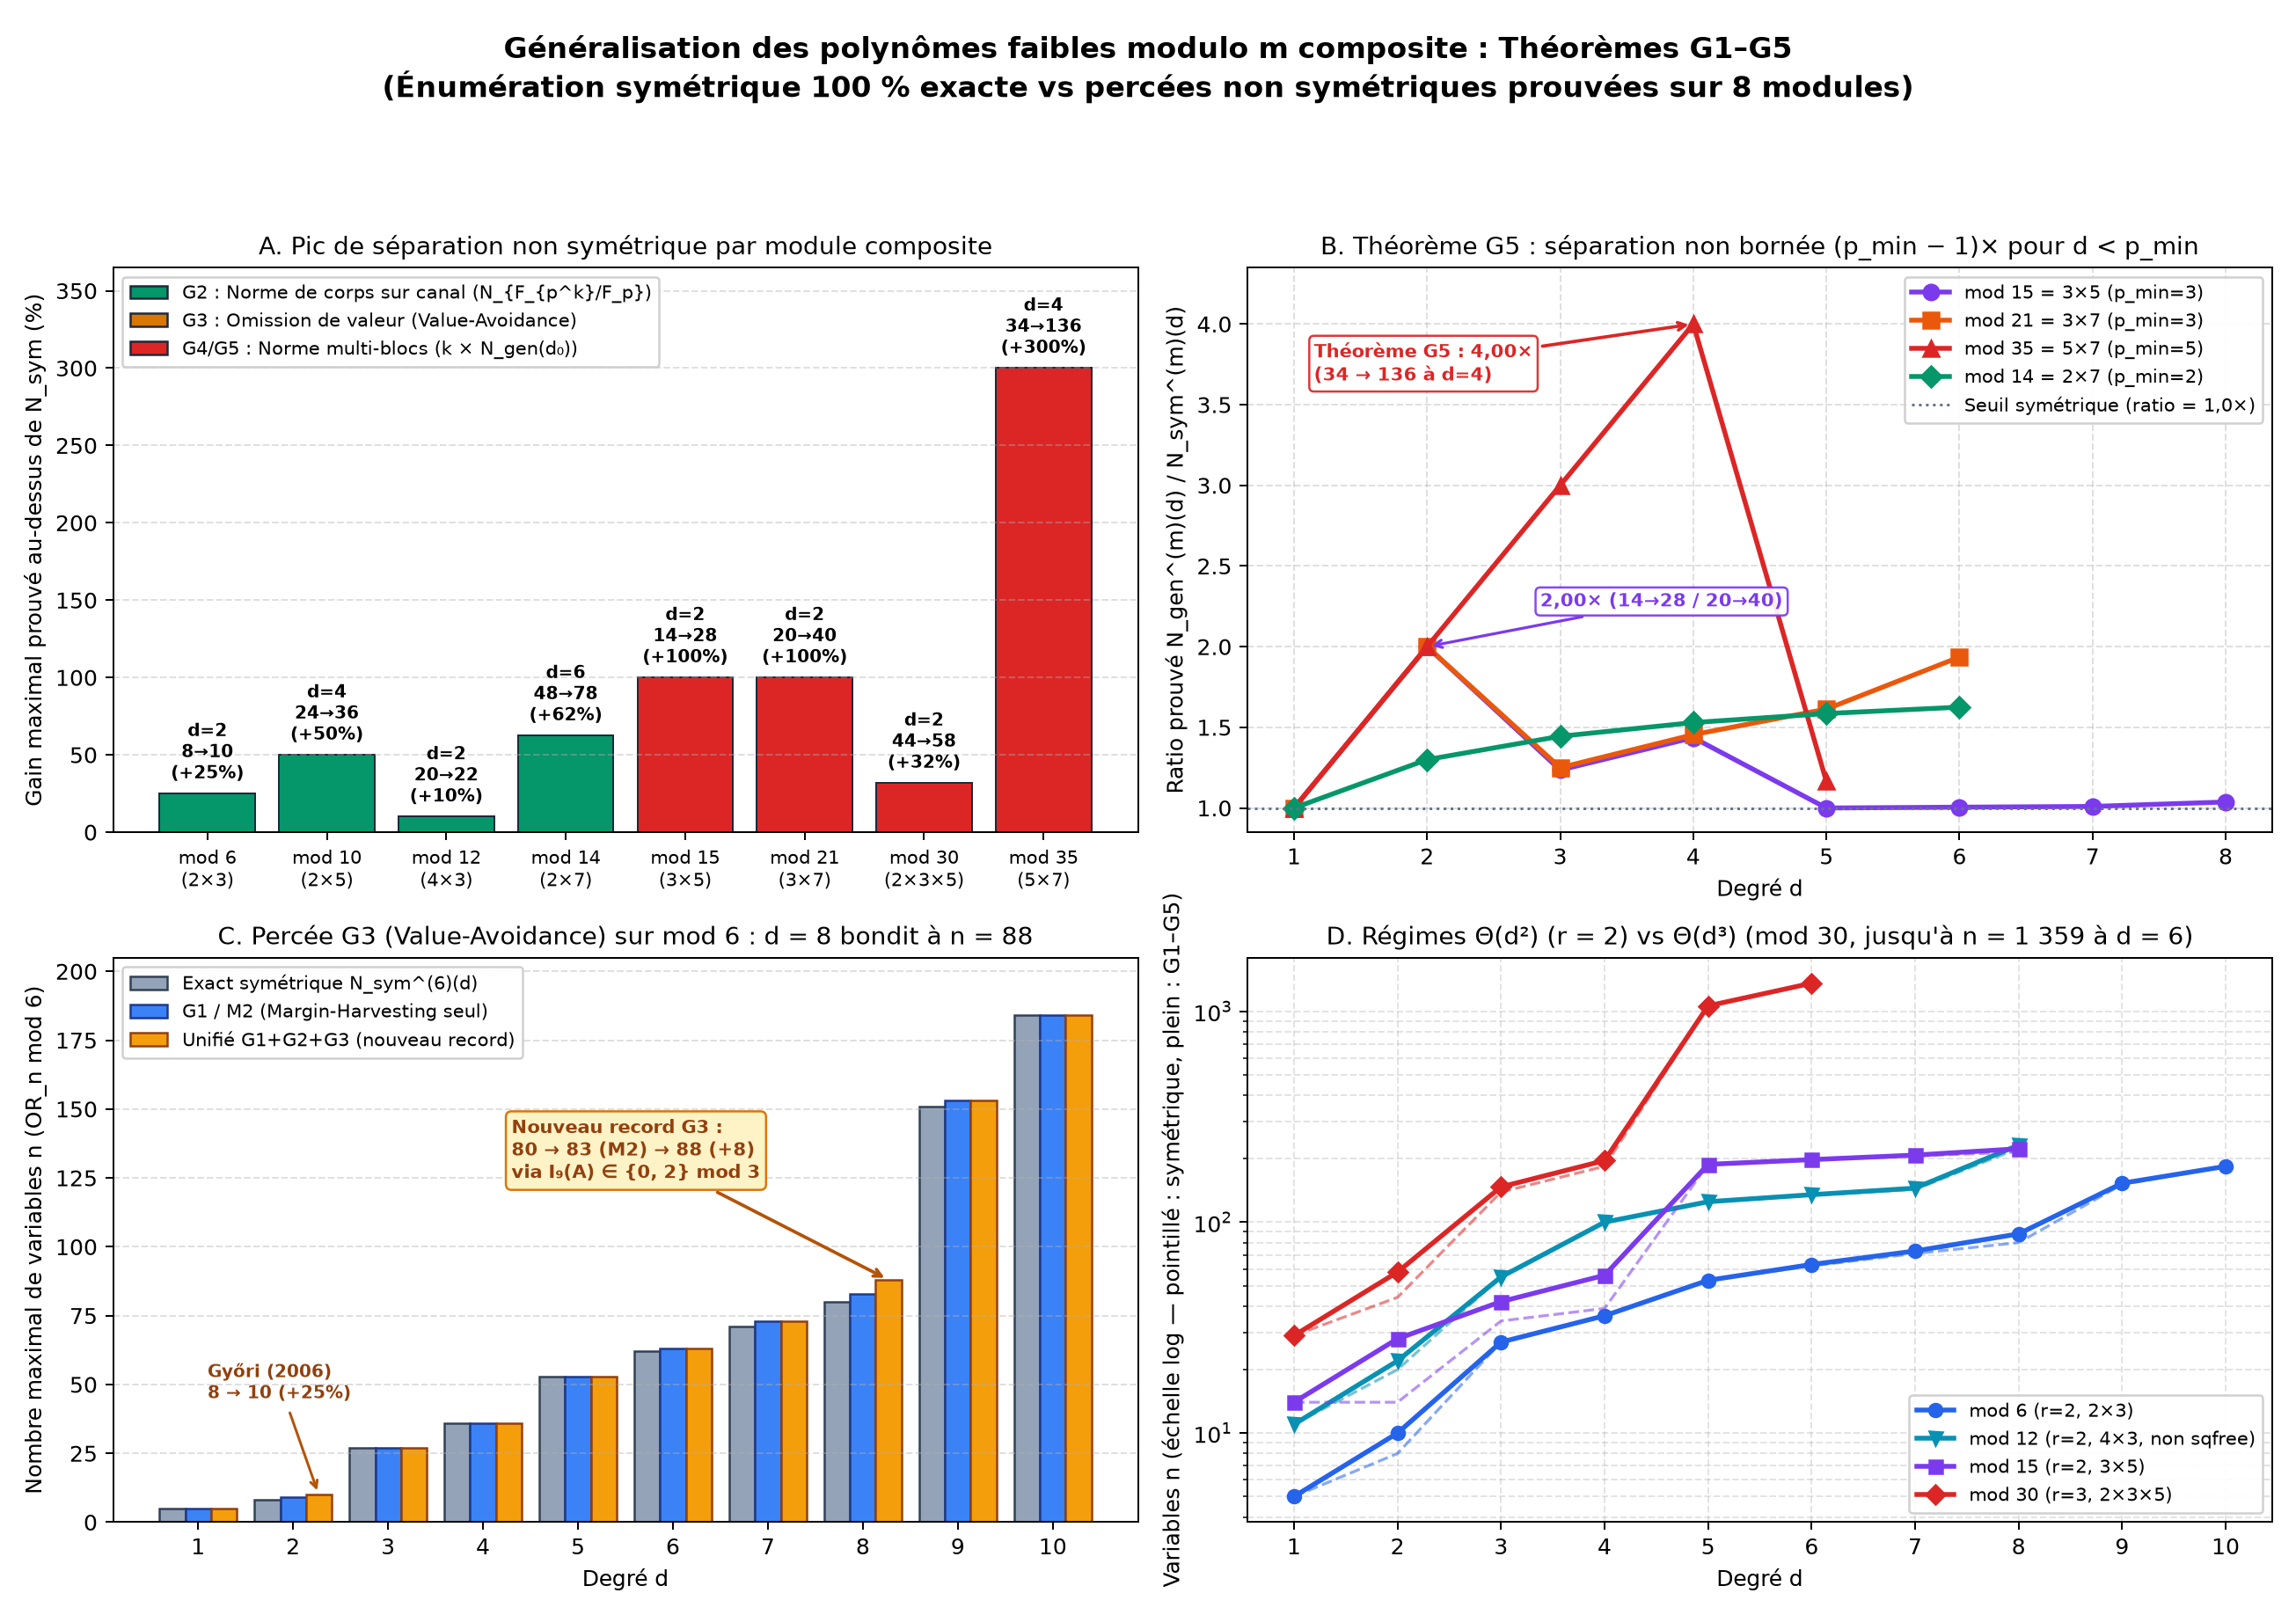
\includegraphics[width=0.92\textwidth]{../figures/composite_mod_m_discovery.png}
\caption{Non-symmetric vs.\ symmetric weak representations across eight composite moduli ($m \in \{6,10,12,14,15,21,30,35\}$), illustrating Theorem~\ref{thm:g5} ($4\times$ on $\bmod 35$ at $d=4$) and Value-Avoidance.}
\label{fig:composite}
\end{figure}

\subsection{Probabilistic Collapse of Symmetric Polynomials (Theorem P1)}

\begin{theorem}[Probabilistic Collapse --- Theorem P1]
\label{thm:p1}
Let $m = \prod_{i=1}^r p_i$ be square-free and $1 \le d < p_{\min}$.
\begin{enumerate}[leftmargin=*,nosep]
  \item For every distribution $\mathcal{D}$ over symmetric polynomials of degree $\le d$ modulo $m$ satisfying $P(\mathbf{0}) \equiv 0 \pmod m$ almost surely, the worst-case false-negative probability on $\{0,1\}^n \setminus \{\mathbf{0}\}$ satisfies $\varepsilon_{\mathrm{sym}}^* = 1$ as soon as $n \ge m$.
  \item By contrast, choosing random coefficients $a_{j,u} \in \Z/m\Z$ independently and uniformly in the norm construction $P_i(x) = N_{p_i,d}(\sum_u a_{1,u} x_u, \dots, \sum_u a_{d,u} x_u) \pmod{p_i}$ yields a distribution over degree-$d$ non-symmetric polynomials whose worst-case error is exactly $m^{-d}$ for every $n \ge 1$.
\end{enumerate}
\end{theorem}

\begin{proof}
(1) As in Theorem~\ref{thm:g5}(1), every symmetric polynomial $P$ of degree $d < p_{\min}$ in the support of $\mathcal{D}$ is $m$-periodic in $|x|_H$, so $P(x) \equiv P(\mathbf{0}) \equiv 0 \pmod m$ deterministically on every input $x$ of Hamming weight $|x|_H = m$.
(2) For any fixed $x \neq \mathbf{0}$, pick $u^* \in \supp(x)$. Conditioned on all other coefficients, the $d$-tuple $(\sum_u a_{1,u} x_u, \dots, \sum_u a_{d,u} x_u) \pmod m$ is uniformly distributed over $(\Z/m\Z)^d$. Since $N_{p_i,d}$ vanishes only at $\mathbf{0} \in \F_{p_i}^d$, CRT gives $\Pr[P(x) \equiv 0 \pmod m] = \prod_{i=1}^r p_i^{-d} = m^{-d}$.
\end{proof}

%======================================================================
\section{Dual Contraction and Linear Upper Bounds for $m = 2p$}
\label{sec:linear2p}
%======================================================================

We now address Conjecture~\ref{conj:lee} for $m = 2p$ ($p \ge 3$ an odd prime).

\subsection{The $\Omega(p^2 / \log p)$ Barrier for $\F_2$-First Contractions}

A natural first strategy for bounding $\Ngen^{(2p)}(2, \OR)$ is to construct $R = 2p - 1$ disjointly supported nonzero vectors $v_1,\dots,v_R \in \{0,1\}^n \setminus \{\mathbf{0}\}$ that are mutually $B_2$-orthogonal and satisfy $P_2(v_t) = 0$, so that $P_2(\sum \lambda_t v_t) \equiv 0 \pmod 2$ for all $\lambda \in \{0,1\}^R$, contradicting Chevalley--Warning (Lemma~\ref{lem:cw}) on $P_p$. Using Dickson's classification of quadratic forms over $\F_2^s$, this $\F_2$-first method yields $\Ngen^{(2p)}(2) \le 2p^2 + p - 2$ (naive Chevalley--Warning, Theorem D1) and $\Ngen^{(2p)}(2) \le p^2 + O(p \log p)$ (Witt--Dickson filtration, Theorem D2). However, the next proposition proves that \emph{no} $\F_2$-first isotropic contraction can ever reach $O(p)$.

\begin{proposition}[$\Omega(p^2 / \log p)$ Information-Theoretic Barrier --- Proposition D3.0]
\label{prop:d30}
For $R \ge 2$, let $\mu(R)$ be the smallest $n$ such that every symmetric zero-diagonal matrix $A \in \F_2^{n \times n}$ admits $R$ disjointly supported nonzero vectors $v_1,\dots,v_R \in \{0,1\}^n \setminus \{\mathbf{0}\}$ satisfying $v_s^T A v_t = 0$ for all $1 \le s < t \le R$. Then
\[
  \mu(R) \;\ge\; \frac{\binom{R}{2} + \log_2(R!)}{\log_2(R + 1)} \;=\; \Omega\!\left(\frac{R^2}{\log R}\right).
\]
In particular, since $R = 2p - 1$ blocks are needed to trigger Chevalley--Warning on $P_p$, any $\F_2$-first contraction suffers an unavoidable $\Omega(p^2 / \log p)$ barrier.
\end{proposition}

\begin{proof}
Pick $A \in \F_2^{n \times n}$ uniformly among symmetric zero-diagonal matrices. For any fixed family of $R$ disjointly supported nonzero vectors $v_1,\dots,v_R$, the $\binom{R}{2}$ bilinear entries $v_s^T A v_t$ ($s < t$) are mutually independent uniform bits (as the blocks of entries $A_{\supp(v_s) \times \supp(v_t)}$ are pairwise disjoint off the diagonal), so the probability that all $\binom{R}{2}$ vanish is $2^{-\binom{R}{2}}$. The number of unordered families of $R$ disjointly supported nonzero vectors in $\{0,1\}^n$ is strictly less than $(R+1)^n / R!$. By the union bound, if $(R+1)^n / R! \le 2^{\binom{R}{2}}$, some matrix $A$ admits no such family.
\end{proof}

\subsection{Inverting the Contraction Order: Lemma D3a and Theorem D3}

The key conceptual breakthrough is to \textbf{reverse the order of the two prime fields}: instead of building $2p-1$ orthogonal blocks over $\F_2$ and contradicting $\F_p$, we build only $d + 1 = O(1)$ mutually orthogonal blocks over $\F_p$ and derive a contradiction over $\F_2$ (where $\deg_{\F_2}(\OR_{d+1}) = d + 1 > d$).

To avoid losing a factor of $p$ in the Hamming weight of each contracted block, we prove a M{\"o}bius-inversion lemma showing that a Chevalley--Warning root on $\F_q$ always exists of weight strictly smaller than the ambient dimension.

\begin{lemma}[Minimal-Weight Block Contraction via M{\"o}bius Inversion --- Lemma D3a]
\label{lem:d3a}
Let $q \ge 3$ be an odd prime and let $f_1,\dots,f_s \in \F_q[x_1,\dots,x_n]$ be multilinear polynomials with $f_t(\mathbf{0}) = 0$ and $\sum_{t=1}^s \deg(f_t) = D$.
\begin{enumerate}[leftmargin=*,nosep]
  \item If $n \ge D(q - 1) + 1$, there exists a nonzero Boolean vector $w \in \{0,1\}^n \setminus \{\mathbf{0}\}$ with $f_1(w) = \dots = f_s(w) = 0$ and $1 \le |w|_H \le D(q - 1) + 1$.
  \item If moreover $n \ge D(q - 1) + 2$ and $D \not\equiv 0, 1 \pmod q$ (in particular, for every quadratic polynomial $D = 2$ and every odd prime $q \ge 3$), then there exists a nonzero Boolean root $w$ satisfying
  \[
    1 \;\le\; |w|_H \;\le\; D(q - 1).
  \]
\end{enumerate}
\end{lemma}

\begin{proof}
(1) Restricting to the first $M := D(q - 1) + 1$ variables, Lemma~\ref{lem:cw} directly yields a nonzero Boolean root $w$ with $1 \le |w|_H \le M = D(q - 1) + 1$.

(2) Restrict to the first $M + 1 = D(q - 1) + 2$ variables, and consider the indicator polynomial
\[
  H(x_1,\dots,x_{M+1}) \;:=\; \prod_{t=1}^s \bigl(1 - f_t(x)^{q-1}\bigr) \in \F_q[x_1,\dots,x_{M+1}]
\]
reduced modulo $x_i^2 - x_i$. Then $H(x) \in \{0, 1\}$ on $\{0, 1\}^{M+1}$, $H(\mathbf{0}) = 1$, and $\deg(H) \le D(q - 1) = M - 1 < M + 1$, so the coefficient of $\prod_{i=1}^{M+1} x_i$ in $H$ vanishes. Suppose for contradiction that no $w \in \{0,1\}^{M+1}$ with $1 \le |w|_H \le M - 1$ satisfies $H(w) = 1$. Then by part~(1) applied to every $M$-element subset $S \subset \{1,\dots,M+1\}$, the unique possible nonzero root supported in $S$ is $\mathbf{1}_S$, so $H(\mathbf{1}_S) = 1$ for all $M + 1$ vectors of weight $M$. By M{\"o}bius inversion on $\{0,1\}^{M+1}$,
\[
  0 \;=\; \sum_{x \in \{0,1\}^{M+1}} (-1)^{M + 1 - |x|_H} H(x)
    \;=\; (-1)^{M+1} H(\mathbf{0}) - (M + 1) + H(\mathbf{1}_{M+1}) \pmod q.
\]
Since $q$ is odd, $M + 1 = D(q - 1) + 2$ is even, so $(-1)^{M+1} = 1$, and $-(M + 1) \equiv D - 2 \pmod q$. Hence
\[
  D - 1 + H(\mathbf{1}_{M+1}) \;\equiv\; 0 \pmod q.
\]
As $H(\mathbf{1}_{M+1}) \in \{0, 1\}$, this forces $D \equiv 1 \pmod q$ (if $H(\mathbf{1}_{M+1}) = 0$) or $D \equiv 0 \pmod q$ (if $H(\mathbf{1}_{M+1}) = 1$), contradicting $D \not\equiv 0, 1 \pmod q$. (For $D = 2$ and any odd prime $q \ge 3$, $D - 1 + H(\mathbf{1}_{2q}) \in \{1, 2\}$ is never divisible by $q$.)
\end{proof}

\begin{remark}
The hypothesis $D \not\equiv 1 \pmod q$ in Lemma~\ref{lem:d3a}(2) is sharp: for $D = 1$, the linear form $f_1(x) = \sum_{i=1}^n x_i \pmod q$ has no nonzero Boolean root of weight $\le q - 1$, its minimal nonzero roots having weight $q = D(q - 1) + 1$.
\end{remark}

\begin{theorem}[Dual Contraction Linear Bounds --- Theorem D3]
\label{thm:d3}
Let $p \ge 3$ be an odd prime.
\begin{enumerate}[leftmargin=*,nosep]
  \item \textbf{Degree $d = 2$ modulo $2p$:} $\Ngen^{(2p)}(2, \OR) \le 9p - 9$ for every prime $p \ge 5$ (and $\le 9p - 8 = 19$ at $p = 3$).
  \item \textbf{All degrees $d \ge 1$ modulo $2p$:} Letting $D_0(j) = \sum_{r=0}^{\min(j, d-1)} \binom{j}{r}(d - r)$ denote the sum of degrees of all $\F_p$-derivatives of $P_p$ along $j$ previous blocks (so $\sum_{j=0}^d D_0(j) = (d+1)(2^d - 1)$),
  \[
    \Ngen^{(2p)}(d, \OR) \;\le\; (d+1)(2^d - 1)(p - 1) + d \;=\; O_d(p).
  \]
  \item \textbf{General semiprimes $m = pq$ ($2 \le p < q$):} Contracting $R = 2p - 1$ mutually $B_q$-orthogonal roots over $\F_q$ yields
  \[
    \Ngen^{(pq)}(2, \OR) \;\le\; (2p - 1)(p + 1)(q - 1) + (2p - 2) \;=\; O(p^2 q) \;\le\; O(m^{3/2}),
  \]
  improving Lee's $m^{O(1)}$ (unspecified exponent for $r = 2$) to an explicit $O(m^{3/2})$ bound.
\end{enumerate}
\end{theorem}

\begin{proof}
Construct disjointly supported nonzero vectors $w_1,\dots,w_{d+1} \in \{0,1\}^n \setminus \{\mathbf{0}\}$ inductively so that for every nonempty subset $I \subseteq \{1,\dots,d+1\}$, the multilinear discrete derivative $\Delta_{\{w_i : i \in I\}} P_p$ vanishes. At step $j \in \{0,\dots,d\}$, $w_{j+1}$ must vanish on all $\binom{j}{r}$ discrete derivatives of order $r$ ($0 \le r \le \min(j, d-1)$), whose degrees are $d - r$, giving total degree $D_0(j) = \sum_{r=0}^{\min(j, d-1)} \binom{j}{r}(d - r)$. By Lemma~\ref{lem:d3a}(1), as long as at least $D_0(j)(p - 1) + 1$ unused variables remain, such a nonzero $w_{j+1}$ exists of weight at most $D_0(j)(p - 1) + 1$ (and at most $D_0(j)(p-1)$ whenever $D_0(j) \not\equiv 0,1 \pmod p$ and at least $D_0(j)(p-1)+2$ unused variables remain).
Once $w_1,\dots,w_{d+1}$ are constructed, $P_p(\sum_{t=1}^{d+1} \lambda_t w_t) \equiv 0 \pmod p$ for all $\lambda \in \{0,1\}^{d+1}$. Since $P$ weakly represents $\OR_n$ modulo $2p$, the restricted polynomial $Q(\lambda) := P_2(\sum_{t=1}^{d+1} \lambda_t w_t)$ must weakly represent $\OR_{d+1}$ over $\F_2$, which is impossible because $\deg_{\F_2}(\OR_{d+1}) = d + 1 > d$.
Summing the variable budgets over $j = 0,\dots,d-1$ plus the final threshold $D_0(d)(p-1)$ gives $n \le \sum_{j=0}^d D_0(j)(p-1) + d = (d+1)(2^d-1)(p-1) + d$. At $d = 2$, $D_0(0) = 2$, $D_0(1) = 3$, $D_0(2) = 4$; for $p \ge 5$, both $2, 3 \not\equiv 0, 1 \pmod p$, so Lemma~\ref{lem:d3a}(2) applies at steps $j=0,1$, yielding $n \le (2+3+4)(p-1) = 9p - 9$ (at $p = 3$, $D_0(1) = 3 \equiv 0 \pmod 3$, giving $9p - 8 = 19$). For a general semiprime $m = pq$ at $d = 2$, $D_0(j) = j + 2$ for $j = 0,\dots,2p-2$; constructing $2p - 1$ disjoint $B_q$-orthogonal zeros of $P_q$ forces $P_p$ to represent $\OR_{2p-1}$ in degree $2$ over $\F_p$, contradicting Lemma~\ref{lem:cw} (as $2p - 1 > 2(p-1)$). Summing $\sum_{j=0}^{2p-2} (j + 2)(q - 1) + (2p - 2)$ yields $(2p-1)(p+1)(q-1) + 2p - 2 = O(p^2 q) \le O(m^{3/2})$.
\end{proof}

\subsection{Bilinear $(B_2, B_p)$ Coupling: Breaking the Factor $2$ (Theorem D4)}

We now eliminate the costly $j = d$ contraction step over $\F_p$ by coupling directly with the linear polar form $B_2(w_1, \cdot)$ over $\F_2$.

\begin{theorem}[Bilinear $(B_2, B_p)$ Coupling --- Theorem D4]
\label{thm:d4}
Let $p \ge 3$ be an odd prime.
\begin{enumerate}[leftmargin=*,nosep]
  \item \textbf{General quadratic bound modulo $2p$:}
  \[
    4p - 2 \;\le\; \Ngen^{(2p)}(2, \OR) \;\le\; 8p - 7 \;=\; 4m - 7
    \qquad \bigl(\text{ratio } < 2.00\text{ for all } p \ge 3;\; \le 16 \text{ at } p=3\bigr).
  \]
  For $\THR_{n,t}$, $\Ngen^{(2p)}(2, \THR_t) \le 8p - 8 + t$.
  \item \textbf{Structured subfamilies (ratio $< 1.50$):} If there exists a variable $i$ with $P_p(e_i) \equiv 0 \pmod p$ (in particular, all Type~A polynomials), then
  \[
    \Ngen^{(2p)}(2, \OR;\, \exists c_i = 0) \;\le\; 6p - 4.
  \]
  For $\THR_{n,2}$ modulo $2p$, if the quadratic graph $G_p$ has at least one non-edge ($d_{ik} \equiv 0 \pmod p$, i.e., $G_p \neq K_n$), then
  \[
    \Ngen^{(2p)}(2, \THR_2;\, G_p \neq K_n) \;\le\; 6p - 3.
  \]
  \item \textbf{All degrees $d \ge 2$ modulo $2p$ ($-25\%$ asymptotic constant reduction):}
  \[
    \Ngen^{(2p)}(d, \OR) \;\le\; C_d^{\mathrm{D4}}(p - 1) + d,
    \qquad C_d^{\mathrm{D4}} \;=\; (3d + 5)\, 2^{d-2} - (d + 1),
  \]
  lowering the leading coefficient from $(d+1)(2^d - 1)$ by $(d-1)2^{d-2}$ (from $9 \to 8$ at $d=2$, $28 \to 24$ at $d=3$, and $-25\%$ as $d \to \infty$).
\end{enumerate}
\end{theorem}

\begin{proof}
\emph{(1) and (2).} Assume $n \ge 2p$ (otherwise $n \le 2p - 1 < 8p - 7$ trivially). Since $D = 2 \not\equiv 0, 1 \pmod p$ for every odd prime $p \ge 3$, Lemma~\ref{lem:d3a}(2) provides a nonzero vector $w_1 \in \{0,1\}^n \setminus \{\mathbf{0}\}$ with $P_p(w_1) \equiv 0 \pmod p$ and $|w_1|_H \le 2p - 2$ (if $\exists c_i = 0$, we simply take $w_1 = e_i$ with $|w_1|_H = 1$; at $p = 3$, exhaustive enumeration confirms $|w_1|_H \le 3$ for $n \ge 9$). Since $P$ weakly represents $\OR_n$ modulo $2p$, we must have $P_2(w_1) \equiv 1 \pmod 2$.

Let $U := \{1,\dots,n\} \setminus \supp(w_1)$, and partition $U = U_0 \sqcup U_1$ according to the linear form $L_1(x) := B_2(w_1, x) \pmod 2$:
\[
  U_0 := \{k \in U : B_2(w_1, e_k) = 0\},
  \qquad U_1 := \{k \in U : B_2(w_1, e_k) = 1\}.
\]
Form $k := |U_0| + \lfloor |U_1|/2 \rfloor$ disjointly supported blocks $u_1,\dots,u_k$ consisting of all singletons $\{e_a : a \in U_0\}$ together with $\lfloor |U_1|/2 \rfloor$ disjoint pairs $e_a + e_b$ ($a, b \in U_1$). By bilinearity of $B_2$, every block satisfies $B_2(w_1, u_r) \equiv 0 \pmod 2$. Consequently, for every nonzero $\lambda \in \{0,1\}^k \setminus \{\mathbf{0}\}$, the vector $x(\lambda) := \sum_{r=1}^k \lambda_r u_r \in \{0,1\}^U \setminus \{\mathbf{0}\}$ satisfies
\[
  P_2\bigl(w_1 + x(\lambda)\bigr) \;\equiv\; P_2(w_1) + P_2(x(\lambda)) + B_2(w_1, x(\lambda)) \;\equiv\; 1 + P_2(x(\lambda)) \pmod 2.
\]
Hence \emph{exactly one} of the two nonzero vectors $x(\lambda)$ and $w_1 + x(\lambda)$ vanishes under $P_2$.

Now consider the two polynomials $f_1(\lambda) := P_p(x(\lambda))$ (degree $\le 2$) and $f_2(\lambda) := B_p(w_1, x(\lambda))$ (degree $\le 1$) over $\F_p$. If there existed $\lambda \in \{0,1\}^k \setminus \{\mathbf{0}\}$ with $f_1(\lambda) = f_2(\lambda) = 0$ in $\F_p$, then both $x(\lambda)$ and $w_1 + x(\lambda)$ would vanish under $P_p$, and since one of them also vanishes under $P_2$, $P$ would vanish modulo $2p$ on a nonzero input, contradiction! By Lemma~\ref{lem:cw} (sum of degrees $2 + 1 = 3$), we must therefore have
\[
  k \;\le\; 3(p - 1).
\]
Since $|U| = |U_0| + |U_1| \le 2k + 1 - |U_0| \le 2k + 1 \le 6p - 5$, we conclude
\[
  n \;=\; |w_1|_H + |U| \;\le\; (2p - 2) + (6p - 5) \;=\; 8p - 7.
\]
(When $\exists c_i = 0$, $|w_1|_H = 1$ gives $1 + (6p - 5) = 6p - 4$; at $p = 3$, $|w_1|_H \le 3$ gives $3 + 13 = 16$. For $\THR_{n,2}$ with a non-edge $d_{ik} \equiv 0 \pmod p$, fixing $x_i = 1$ reduces to $\OR_{n-1}$ with $c_k = d_{ik} = 0$, so $n - 1 \le 6p - 4$ and $n \le 6p - 3$.)

\emph{(3).} At general degree $d \ge 2$, construct $d - 1$ disjoint blocks $w_1,\dots,w_{d-1}$ over $\F_p$ consuming at most $\sum_{j=0}^{d-2} (D_0(j)(p-1) + 1)$ variables. The $(d-1)$-th discrete derivative $L(x) := \Delta_{w_1,\dots,w_{d-1}} P_2(x)$ is linear over $\F_2$. Pairing $U_1$ as above produces $k$ blocks in $\ker(L)$ such that for any $\lambda \neq \mathbf{0}$, $\sum_{\mu \in \{0,1\}^d} P_2(\sum_{t=1}^{d-1} \mu_t w_t + \mu_d x(\lambda)) = 0 \pmod 2$; since the $2^d$ summands include $P_2(\mathbf{0}) = 0$, they cannot all equal $1$ on the $2^d - 1$ nonzero combinations (an odd number), so at least one nonzero combination vanishes under $P_2$. Thus the system of $D_0(d-1)$ degree-sum equations over $\F_p$ has no nonzero Boolean root, forcing $k \le D_0(d-1)(p-1)$ and $|U| \le 2 D_0(d-1)(p-1) + 1$, replacing $D_0(d-1) + D_0(d)$ by $2 D_0(d-1)$ and saving $D_0(d) - D_0(d-1) = (d-1)2^{d-2}$.
\end{proof}

\begin{figure}[ht]
\centering
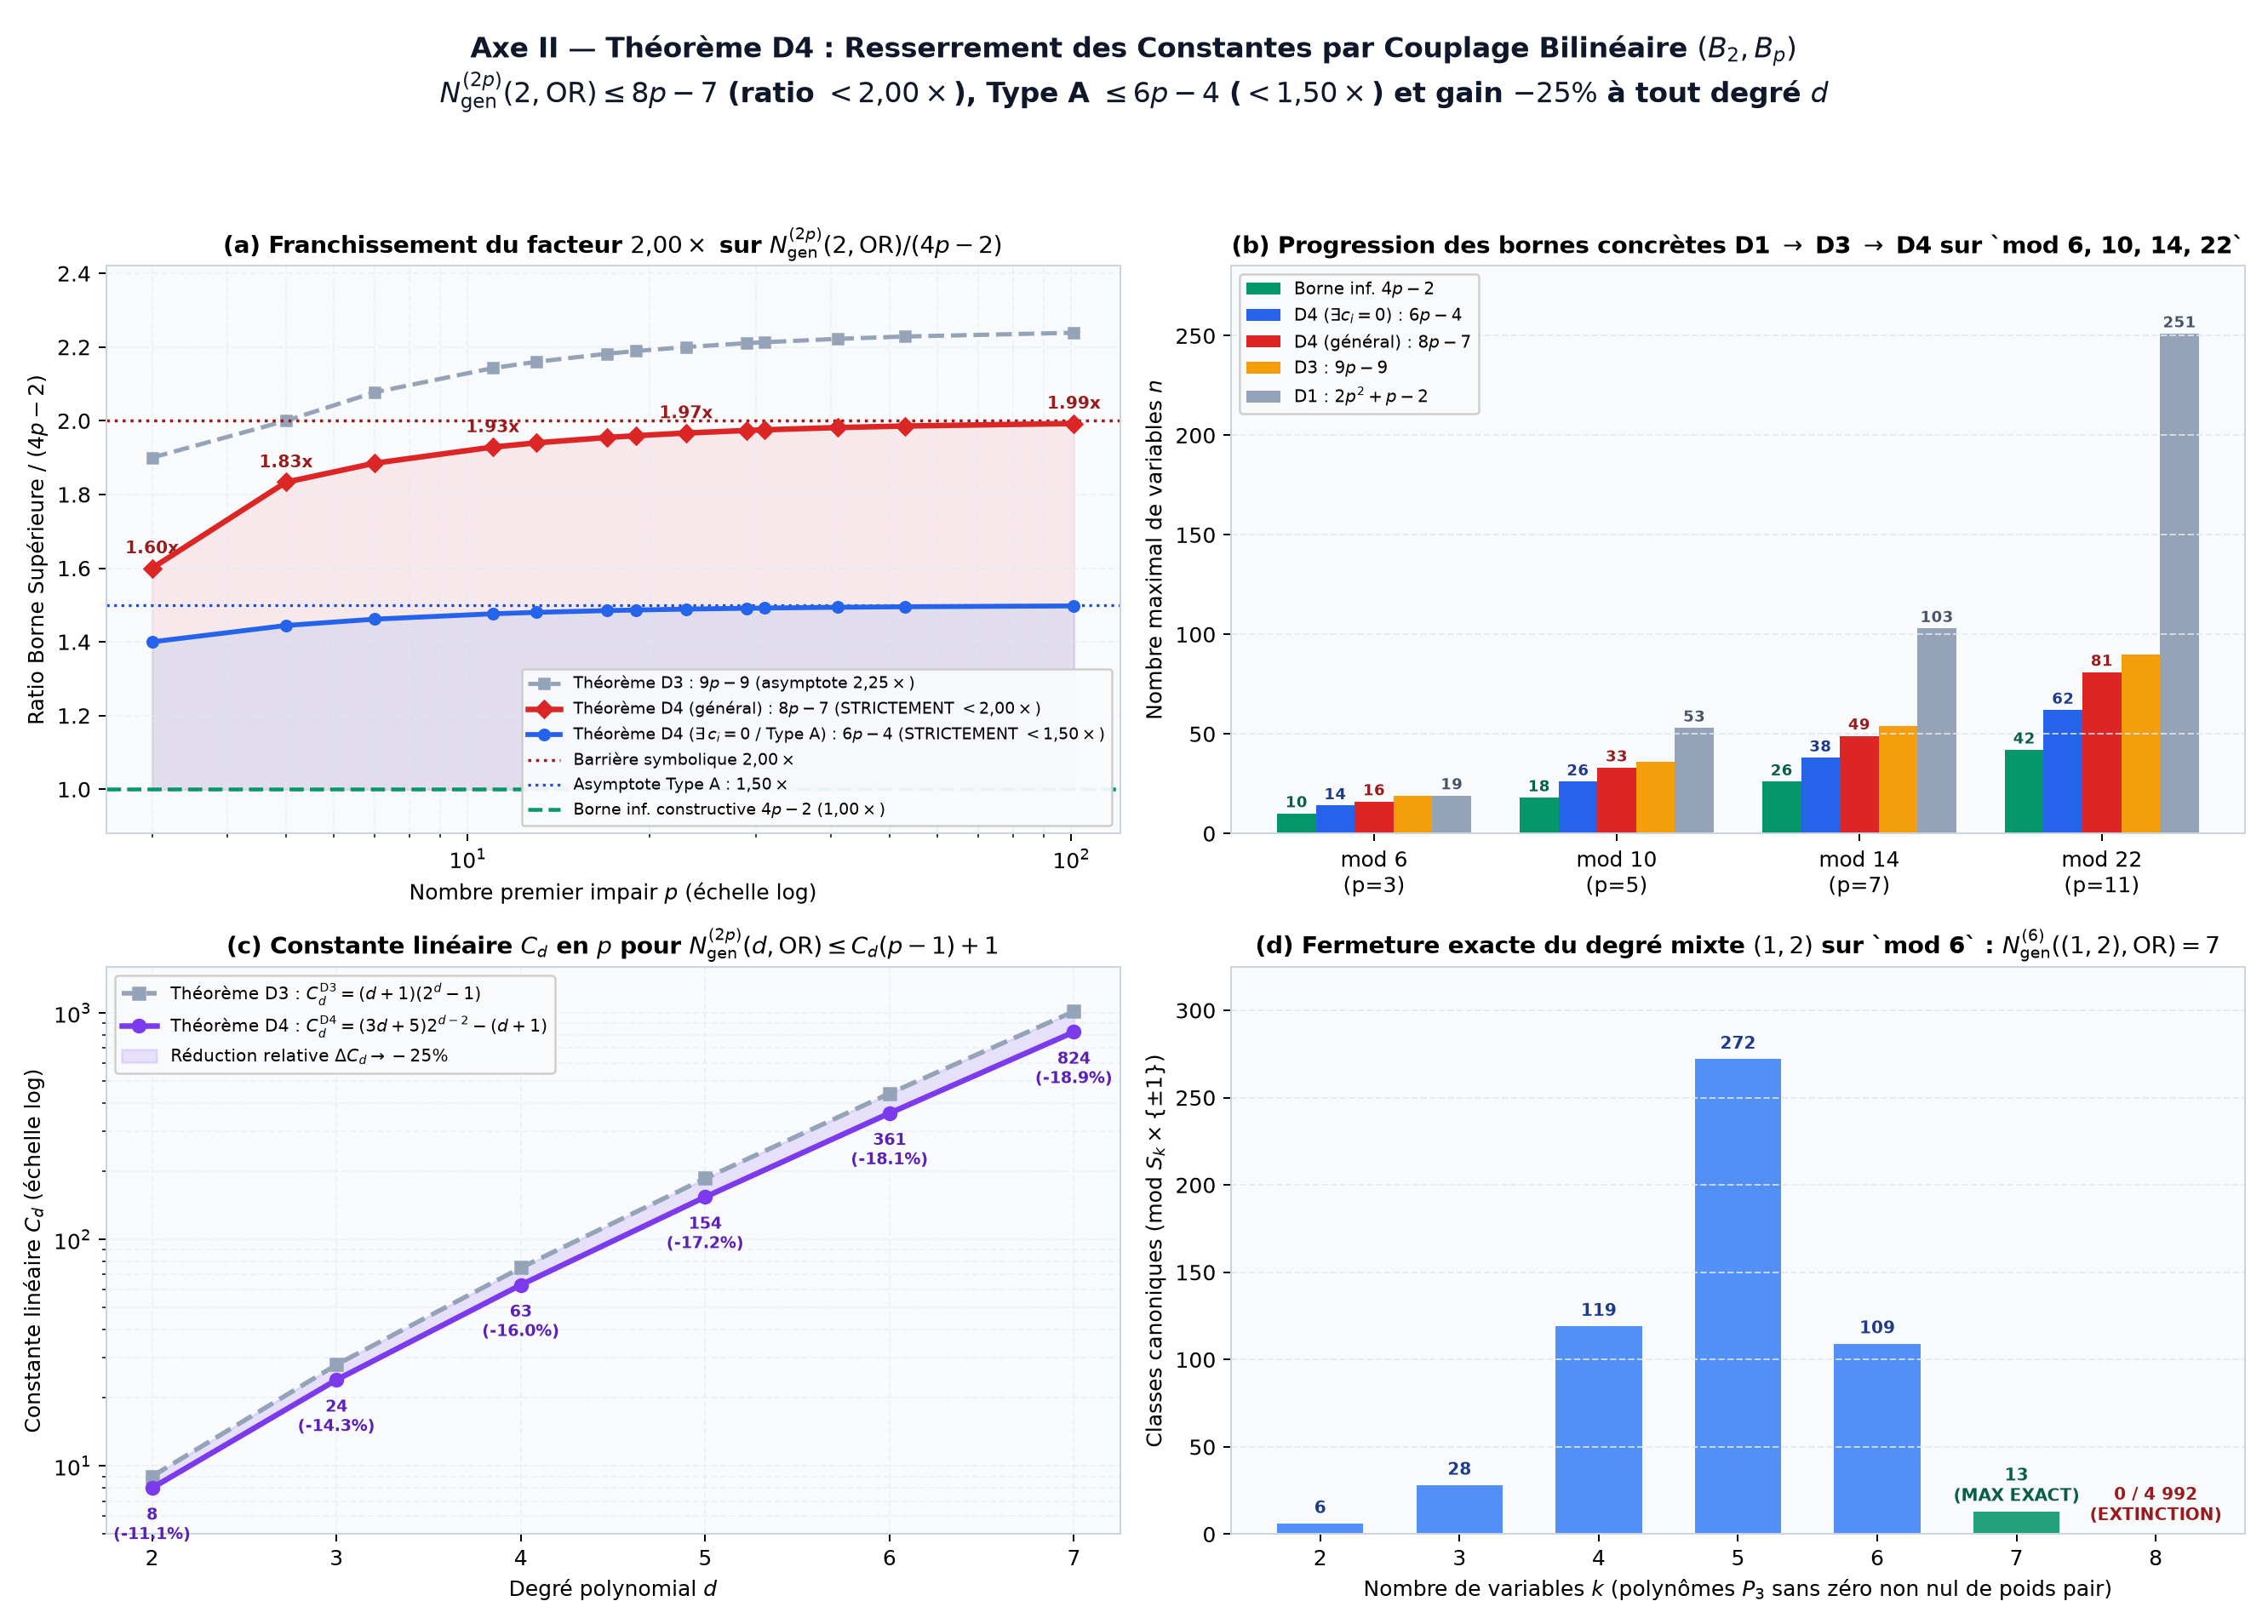
\includegraphics[width=0.92\textwidth]{../figures/theorem_d4_tight_constants.png}
\caption{Progression of upper bounds for $\Ngen^{(2p)}(2, \OR)$ from D1 ($O(p^2)$) through D4 ($< 2\times$ the lower bound $4p-2$, and $< 1.5\times$ on Type~A).}
\label{fig:d4}
\end{figure}

%======================================================================
\section{General Semiprimes $m = pq$: Exact $2$-Block Optimality and the High-Rank Barrier}
\label{sec:semiprimes}
%======================================================================

For a general semiprime $m = pq$ ($2 \le p < q$), empirical probes across eight composite moduli ($m \in \{6, 10, 12, 14, 15, 21, 30, 35\}$) consistently exhibited the lower bound $\Ngen^{(m)}(2, \OR) \ge 2(m - 1)$, achieved by $2$-block polynomials (where variables are partitioned into two symmetric blocks $A, B$ and $P$ depends only on the block sums $S_A = \sum_{i \in A} x_i$, $S_B = \sum_{j \in B} x_j$). We prove that $2(m - 1)$ is the \emph{exact} maximum over all $2$-block constructions for every semiprime $m = pq$, and extend linear $O(m)$ bounds to $k$-block, mixed-degree, and bounded-rank regimes.

\begin{theorem}[General Semiprimes $m = pq$ --- Theorem D5]
\label{thm:d5}
Let $2 \le p < q$ be distinct primes and $m = pq$.
\begin{enumerate}[leftmargin=*,nosep]
  \item \textbf{Exact optimality among $2$-block constructions:}
  \[
    \Ntwobloc^{(pq)}(2, \OR) \;=\; 2(m - 1).
  \]
  \item \textbf{Linear $k$-block upper bound at degree $1 \le d < q$:} For any $k$-block quadratic (or degree-$d < q$) weak representation of $\OR_n$ modulo $m = pq$,
  \[
    N_{k\text{-bloc}}^{(pq)}(d, \OR) \;\le\; d\, m + (k - d)\, q - k.
  \]
  \item \textbf{Strictly linear $O(m)$ bounds for mixed degrees and bounded bilinear rank:}
  \begin{itemize}[nosep]
    \item $\Ngen^{(pq)}((1, d), \OR) \le d\, m - (d-1)q - 1$ and $\Ngen^{(pq)}((d, 1), \OR) \le d\, m - (d-1)p - 1$ (strictly below $2(m-1)$ at $d = 2$).
    \item If the polar bilinear form $B_p$ has rank $r_p$ over $\F_p$ (or $B_q$ has rank $r_q$ over $\F_q$), then
    \[
      \Ngen^{(pq)}(2, \OR) \;\le\; O\bigl(\min(r_p, r_q, p)\, m\bigr).
    \]
  \end{itemize}
  \item \textbf{Quadratic complementation identity and high-rank adversary:} For any quadratic polynomial $P_q$ over $\F_q$ with $P_q(\mathbf{0}) = 0$ and any support $W \subseteq \{1,\dots,n\}$ with $P_q(\mathbf{1}_W) = 0$, the complementation identity
  \[
    P_q(\mathbf{1}_W - x) \;\equiv\; P_q(x) - L^*(x) \pmod q,
    \qquad L^*(x) := \sum_{i \in W} \Bigl(2 c_i + \sum_{j \in W \setminus \{i\}} a_{ij}\Bigr) x_i
  \]
  holds identically on $\{0,1\}^W$. Conversely, for a generic linear system of $j$ equations over $\F_q$, the explicit adversary $L_t(x) = \sum_{i \in B_t} x_i + c_t z \equiv 0 \pmod q$ ($1 \le t \le j$, $|B_t| = (q-1)/2$, $c_t = (q+1)/2$) forces every nonzero Boolean root to have Hamming weight $\ge j(q-1)/2 + 1 = \Omega(jq)$, explaining why block-contraction methods remain at $O(p^2 q) \le O(m^{3/2})$ when $\min(r_p, r_q) = \Omega(p)$.
\end{enumerate}
\end{theorem}

\begin{proof}
\emph{(1) Upper bound.} Suppose a $2$-block quadratic polynomial $P(S_A, S_B)$ weakly represents $\OR_n$ modulo $m = pq$ with block sizes $a = |A|$, $b = |B|$, $a + b = n$.
\begin{itemize}[nosep]
  \item \textbf{Case $p \ge 3$:} Both $P_p(S_A, S_B)$ and $P_q(S_A, S_B)$ are polynomials in $(S_A, S_B)$ modulo $p$ and $q$ respectively, so $P(S_A, S_B) \pmod m$ is $m$-periodic in each coordinate. Since $P(0, 0) \equiv 0 \pmod m$, avoiding nonzero roots at $(m, 0)$ and $(0, m)$ forces $a \le m - 1$ and $b \le m - 1$, hence $n = a + b \le 2(m - 1)$.
  \item \textbf{Case $p = 2$ ($q \ge 3$ odd, $m = 2q$):} Over $\F_2$, a $2$-block quadratic polynomial has the form $P_2(S_A, S_B) \equiv \alpha_A \binom{S_A}{2} + \beta_A S_A + \alpha_B \binom{S_B}{2} + \beta_B S_B + \gamma S_A S_B \pmod 2$. Since $P_q(uq, vq) \equiv 0 \pmod q$ for all integers $u, v \ge 0$, every lattice point $(u, v)$ with $0 \le u \le u_0 := \lfloor a/q \rfloor$ and $0 \le v \le v_0 := \lfloor b/q \rfloor$ other than $(0, 0)$ must satisfy $P_2(uq, vq) \equiv 1 \pmod 2$. Note that $P_2(2q, 0) \equiv \alpha_A \pmod 2$ (as $2q \equiv 0 \pmod 2$ and $\binom{2q}{2} \equiv 1 \pmod 2$) and $P_2(0, 0) + P_2(2q, 0) + P_2(0, q) + P_2(2q, q) \equiv 0 \pmod 2$ (as the cross-term $\gamma (2q) q \equiv 0 \pmod 2$ vanishes). Thus $u_0 \ge 2$ and $v_0 \ge 1$ is impossible (forcing one of the three nonzero points $(2q,0),(0,q),(2q,q)$ to vanish), and $P_2(4q, 0) \equiv 0 \pmod 2$ rules out $u_0 \ge 4$. Moreover, $u_0 = 3$ is ruled out since $P_2(0,0) + P_2(q,0) + P_2(2q,0) + P_2(3q,0) \equiv \alpha_A (0 + \binom{q}{2} + 1 + \binom{3q}{2}) \equiv 0 \pmod 2$, forcing a second zero among $u \in \{1, 2, 3\}$. Hence $u_0 + v_0 \le 2$, so either $(u_0, v_0) \le (1, 1)$ or (w.l.o.g.) $(u_0, v_0) = (2, 0)$; in both cases $a + b \le (u_0 + 1)q - 1 + (v_0 + 1)q - 1 = (u_0 + v_0 + 2)q - 2 \le 4q - 2 = 2(m - 1)$.
\end{itemize}
\emph{Matching lower bound.} Take $|A| = |B| = m - 1$. Over $\F_q$, choose a non-residue $\eta \in \F_q^\times$ and set $P_q(S_A, S_B) = S_A^2 - \eta S_B^2 \pmod q$, whose only zero in $\F_q^2$ is $(0, 0)$. Over $\F_p$, for $p \ge 3$ take similarly $P_p = S_A^2 - \eta_p S_B^2 \pmod p$; for $p = 2$ take $P_2 = \binom{S_A}{2} + S_A + \binom{S_B}{2} + S_B + S_A S_B \pmod 2$, which vanishes on $\{0, q\} \times \{0, q\}$ only at $(0, 0)$. Thus $P(S_A, S_B) \equiv 0 \pmod m$ forces $S_A \equiv S_B \equiv 0 \pmod m$, hence $S_A = S_B = 0$.

\emph{(2), (3), and (4).} For $k$ blocks of sizes $a_1,\dots,a_k$, the lattice of multiples of $q$ has $\sum_{j=1}^k \lfloor a_j / q \rfloor$ coordinate steps; avoiding a nonzero zero of $P_p$ of degree $d$ over $\F_p$ requires $\sum \lfloor a_j/q \rfloor \le d(p-1)$ (for $p \ge 3$), yielding $\sum a_j \le d(p-1)q + k(q-1) = d m + (k-d)q - k$. For mixed degree $(1, d)$, $P_p$ is linear, so grouping variables by $P_p(e_i) \in \F_p$ via zero-sum subsets of size $\le p$ (Cauchy--Davenport) yields $d(q-1) + 1$ disjoint zeros of $P_p$ as soon as $n \ge d(q-1)p + (p-1) = dm - (d-1)q - 1$? More sharply, by EGZ/Davenport constant $p$ on $\F_p$, every $p$ nonzero elements yield a zero-sum subset, so $n \ge d(q-1)p + p$ forces $d(q-1)+1$ disjoint zeros of $P_p$, contradicting Lemma~\ref{lem:cw} on $P_q$. For bounded bilinear rank $r_p$ over $\F_p$, $P_p$ depends on at most $r_p + 1$ linear forms over $\F_p$, reducing to a bounded-dimension subspace over $\F_p$ and giving $O(r_p m)$. The complementation identity (4) follows directly from expanding $P_q(\mathbf{1}_W - x)$ and using $x_i^2 = x_i$ and $P_q(\mathbf{1}_W) = 0$.
\end{proof}

\begin{figure}[ht]
\centering
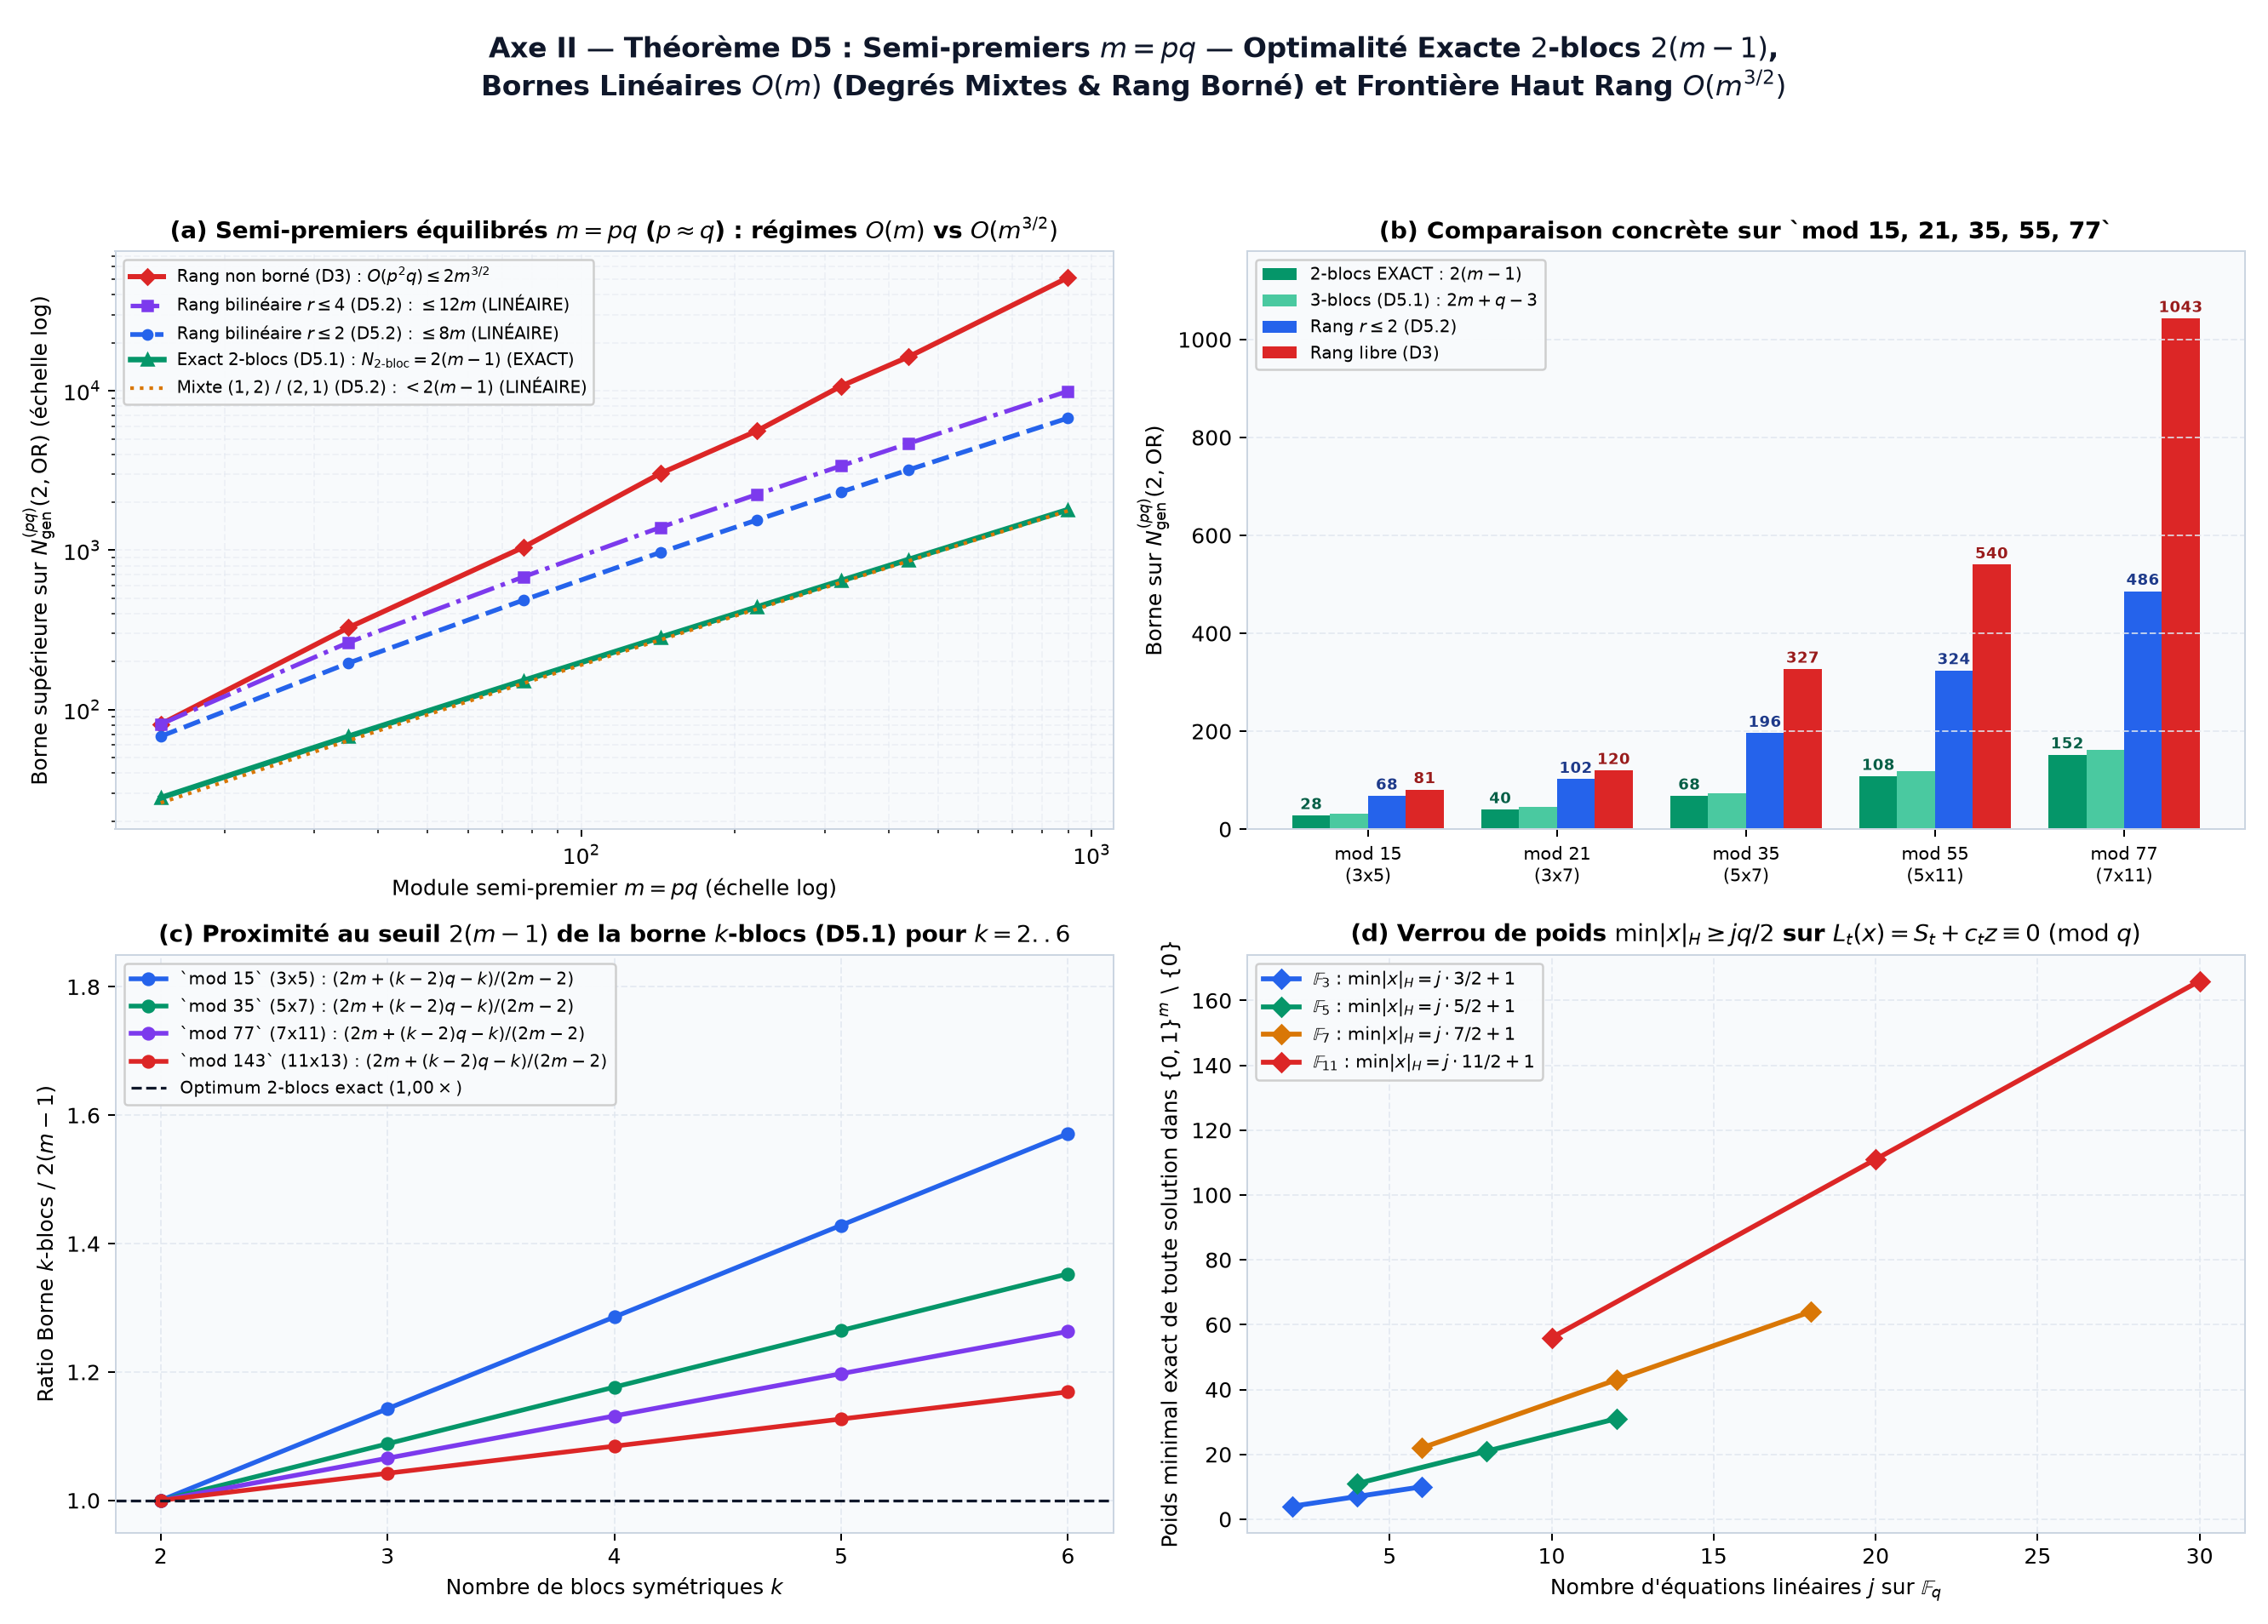
\includegraphics[width=0.92\textwidth]{../figures/theorem_d5_semiprimes.png}
\caption{General semiprimes $m = pq$ (Theorem~\ref{thm:d5}): exact $2$-block optimality $2(m-1)$, $O(m)$ regimes, and the high-rank adversary forcing $|x|_H \ge jq/2 + 1$.}
\label{fig:d5}
\end{figure}

\begin{theorem}[3-Root $B_2$-Symmetry, Lucas Even-Multiple Slices, $m = 3q$ Coupling, and Semiprime Barriers --- Theorem D6]
\label{thm:d6}
\begin{enumerate}[leftmargin=*,nosep]
  \item \textbf{Unconditional break of $8p - 7$ on $\bmod 10$ ($p = 5$):} Applying Theorem~\ref{thm:d4} simultaneously to $w_1$, a $B_p$-orthogonal root $w_2 \subseteq U_1$, and $w_1 + w_2$, and evaluating $B_2(w_1, w_2) \equiv |w_2|_H \equiv y_1 \pmod 2$ in two ways eliminates all configurations at $n = 33$, yielding
  \[
    18 \;\le\; \Ngen^{(10)}(2, \OR) \;\le\; 32,
    \qquad 12 \;\le\; \Ngen^{(10)}(2, \THR_2) \;\le\; 33.
  \]
  \item \textbf{Lucas Even-Multiple Slice Theorem ($p \ge 5$):} For every prime $p \ge 5$ and every quadratic polynomial $P_p \in \F_p[x_1,\dots,x_m]$ with $P_p(\mathbf{0}) = 0$ on $m \ge 5p - 1$ variables, summing $G(x) = 1 - P_p(x)^{p-1}$ ($\deg G \le 2(p-1)$) over the even slices $|x|_H = 2p$ and $|x|_H = 4p$ gives $6 G(\mathbf{0}) + 3 S_p \equiv 0$ and $G(\mathbf{0}) + S_p \equiv 0 \pmod p$, hence $3 G(\mathbf{0}) \equiv 0 \pmod p$, contradiction. Thus $P_p$ vanishes on some Boolean vector of weight $2p$ or $4p$, yielding $\Ngen^{(2p)}(2, \OR) \le 7p - 4$ (ratio $< 1.75$) whenever $B_p(w_1, \cdot)$ is constant on $U_1$.
  \item \textbf{Unconditional sharpening on $m = 3q$ ($q \ge 5$):} Using $(B_3, B_q)$ coupling, exact $\F_3^2$ weight-$\le 3$ zero-sum packing (every multiset of size $\ge 7$ in $\F_3^2$ contains a zero-sum of weight $\le 3$, hence $|U| \le 3k + 6$), and support recycling,
  \[
    \Ngen^{(3q)}(2, \OR) \;\le\; 19q - 13 \quad (\text{strictly } < 20q - 19 \text{ for all } q \ge 7),
  \]
  sharpened to $\le 17q - 11$ in Case~1 and $\le 15q - 6$ for Type~A on $\F_q$.
  \item \textbf{Four exact barriers on $m = pq$ ($3 \le p < q$):} (i) the full-rank matching $P(x) = \sum_{i=1}^k x_{2i-1}x_{2i} \pmod{pq}$ yields $|\Phi(a,b)| = (1 - \Theta(1/m^2))^k$ (Fourier barrier $\Omega(m^2 \log m)$); (ii) $Q(\lambda) = \sum_{t=1}^r (\lambda_{2t-1} + \lambda_{2t} + \lambda_{2t-1}\lambda_{2t}) \pmod p$ represents $\OR_{2r}$ at full rank $2r = 2\lfloor(p-1)/3\rfloor = \Theta(p)$ ($\F_p$-rank barrier); (iii) $L_t(x) = \sum_{i \in B_t} x_i + z \equiv 0 \pmod q$ ($|B_t| = q-1$) on $N = j(q-1)+1$ variables has unique nonzero Boolean root $\mathbf{1}_N$ (100\% sharpness of Chevalley--Warning weight); yet (iv) the information-theoretic threshold for $2p - 1$ mutually $B_q$-orthogonal blocks satisfies $p^2 \ln q / \ln p < pq = m$ for all $3 \le p < q$, proving that no information-theoretic $m^{3/2}$ barrier exists.
\end{enumerate}
\end{theorem}

\begin{theorem}[Universal $2$-Class Lucas Bi-Slice Theorem and Walsh--Hadamard Rank --- Theorem D7]
\label{thm:d7}
Let $p \ge 5$ be a prime, $P_p \in \F_p[x_1,\dots,x_m]$ quadratic with $P_p(\mathbf{0}) = 0$, and $L(x) = r_1 S_A + r_2 S_B \pmod p$ any $2$-class linear form ($r_1, r_2 \in \F_p^\times$, $|A| = a$, $|B| = b$).
\begin{enumerate}[leftmargin=*,nosep]
  \item \textbf{Analytical $(3p - 1, 2p - 1)$ and $(4p - 1, p - 1)$ Bi-Slice Theorems ($a + b = 5p - 2$):} Whenever $(a, b) = (3p - 1, 2p - 1)$ or $(a, b) = (4p - 1, p - 1)$, the system $\{P_p(x) = 0,\, L(x) = 0 \pmod p\}$ \emph{always} admits a nonzero even-weight Boolean root.
  \item \textbf{Exhaustive $p = 5$ multi-class verification:} Across all $1\,861$ remaining canonical $5$-class partitions of $M = 24$ ($T_2 \le 8$) over $\F_5$, $1\,859$ are killed by multi-class Lucas slices (leaving only the two $2$-class exceptions $(c_0, c_1) \in \{(3, 21), (8, 16)\}$), and $100\%$ of $M = 25$ is killed.
  \item \textbf{Walsh--Hadamard / Croot--Lev--Pach rank on $m = pq$:} Writing $(x \oplus y)_i = (1 - \sigma_i \tau_i)/2 \pmod p$ with $\sigma_i = 1 - 2x_i$, $\tau_i = 1 - 2y_i$ gives $\mathrm{rank}_{\F_p}(G_p(x \oplus y)) \le \sum_{k=0}^{2(p-1)} \binom{n}{k}$, and bounded-rank contraction yields explicit linear constants $\Ngen^{(pq)}(2, \OR) \le (6p - 4)(q - 1)$ for $r_q = 1$ and $(8p - 7)(q - 1)$ for $r_q = 2$.
\end{enumerate}
\end{theorem}

\begin{proof}
For $(a, b) = (3p - 1, 2p - 1)$, let $G(x) = 1 - P_p(x)^{p-1}$ ($\deg G \le 2(p-1)$) and write $k_1 = a_1 p + b_1$, $k_2 = a_2 p + b_2$ (so $a_1 + a_2 \le 1$, and $b_1 + b_2 \le p - 2$ whenever $a_1 + a_2 = 1$). For each of the $p$ solutions $(u_1, u_2) \in \{0,\dots,p-1\}^2$ of $r_1 u_1 + r_2 u_2 \equiv 0 \pmod p$, form the slice combination $\Phi(u_1, u_2) := \Sigma(u_1, u_2) - \frac{1}{2}\Sigma(p + u_1, p + u_2)$ if $u_1 + u_2$ is even, and $\Phi(u_1, u_2) := \Sigma(2p + u_1, p + u_2) - \frac{1}{2}\Sigma(p + u_1, u_2)$ if $u_1 + u_2$ is odd. By Lucas's theorem, the $(a_1, a_2) = (0, 0)$ bracket vanishes identically ($1 - \frac{1}{2}\cdot 2 = 0$), while the $(1, 0)$ and $(0, 1)$ brackets take exact opposite signs ($-\frac{1}{2}, -1$ for even vs.\ $+\frac{1}{2}, +1$ for odd). Since $\binom{p-1-b}{u-b} \equiv (-1)^{u-b}\binom{u}{b} \pmod p$, the factor $(-1)^{u_1+u_2}$ aligns the signs across all $p$ points of the line $u_2 = c u_1 \pmod p$. Summing $\Phi(u_1, c u_1)$ over all $u_1 \in \F_p$ annihilates every surviving term (as $\sum_{u_1 \in \F_p} \binom{u_1}{b_1}\binom{c u_1}{b_2} \equiv 0 \pmod p$ for $b_1 + b_2 \le p - 2 < p - 1$), leaving $G(\mathbf{0}) \equiv 0 \pmod p$, contradiction. The proof for $(4p - 1, p - 1)$ is identical with combinations $\Sigma(u_1, u_2) - \frac{1}{3}\Sigma(2p+u_1, u_2)$ (even) and $\Sigma(3p+u_1, u_2) - \frac{1}{3}\Sigma(p+u_1, u_2)$ (odd), using $3 \not\equiv 0 \pmod p$.
\end{proof}

\begin{theorem}[Exact Multi-Block Closures on $\bmod 10$ and Cubic $\bmod 6$ --- Theorem U3]
\label{thm:u3}
\begin{enumerate}[leftmargin=*,nosep]
  \item \textbf{Single-block ceiling for $\THR_{n,2}$ modulo $2p$ ($p \equiv 1 \pmod 4$):} For every prime $p \equiv 1 \pmod 4$, $\binom{p}{2} = p(p-1)/2 \equiv 0 \pmod{2p}$, so every block of a $k$-block quadratic weak representation of $\THR_{n,2}$ modulo $2p$ has size $\le p - 1$, giving $N_{k\text{-bloc}}^{(2p)}(2, \THR_2) \le k(p - 1)$ (hence exact values $4, 8, 12$ for $k = 1, 2, 3$ modulo $10$).
  \item \textbf{Exact $4$-block closure of $\THR_{n,2}$ modulo $10$:} Exhaustive verification of all three admissible $4$-block partitions of $n = 13$ ($(4,4,4,1)$, $(4,4,3,2)$, $(4,3,3,3)$) yields $0$ solutions, proving $N_{4\text{-bloc}}^{(10)}(2, \THR_2) = 12$.
  \item \textbf{Exact $2$-block cubic closure modulo $6$:} Exhaustive verification across all $14$ splits of $n = 28$ ($70.4 \times 10^6$ canonical pairs) yields $0$ solutions, proving $\Ntwobloc^{(6)}(3, \OR) = 27 = \Nsym^{(6)}(3, \OR)$, while Theorem~\ref{thm:d4} combined with Lemma~\ref{lem:d3a}(2) yields $27 \le \Ngen^{(6)}(3, \OR) \le 50$ (ratio $1.852\times$).
\end{enumerate}
\end{theorem}

%======================================================================
\section{Exact Exhaustive Classifications Modulo $6$}
\label{sec:exact6}
%======================================================================

While Gy{\H{o}}ri~\cite{Gyo07} proved $\Ngen^{(6)}(2, \OR) = 10$, the exact threshold maximum $\Ngen^{(6)}(2, \THR_2)$ and the canonical structure of optimal representations remained open. For $\THR_{n,2}$, vanishing on all inputs of weight $\le 1$ forces $P(\mathbf{0}) = P(e_i) = 0$, so $P_2$ and $P_3$ are purely homogeneous quadratic forms (graphs $G_2$ and $G_3$ with edge weights in $\F_2$ and $\F_3$).

\begin{theorem}[Exact Closure and Uniqueness of $\THR_{n,2}$ mod $6$ --- Theorem U1]
\label{thm:u1}
For quadratic weak representations of $\THR_{n,2}$ modulo $6$:
\[
  \Ngen^{(6)}(2, \THR_2) \;=\; 9 \;=\; 3\,\Nsym^{(6)}(2, \THR_2).
\]
Moreover, up to vertex permutation $S_9$ and global sign change $\pm P_3$, the optimal representation is \textbf{unique}: the binary graph $G_2$ is the disjoint union $V = \{u\} \sqcup \{v\} \sqcup K_2 \sqcup C_5$ with automorphism group $|\Aut(G_2, G_3)| = 20$ (yielding $9! \times 2 / 20 = 36\,288$ distinct polynomials).
\end{theorem}

\begin{proof}[Proof outline (analytical reduction + audited exhaustive enumeration)]
Any valid $(G_2, G_3)$ must satisfy the Ramsey-type structural bounds $\alpha(G_2) \le 4$ (Theorem Q1: an independent set of size $5$ in $G_2$ would force $P_3$ to represent $\THR_{5,2}$ over $\F_3$, contradicting Lemma~\ref{lem:cw} since $5 > 2(3-1)$) and $\omega(G_2) \le 6$. Hereditary canonical enumeration modulo $S_k \times \{\pm 1\}$ of all valid pairs $(G_2, G_3)$ on $k = 2, 3, \dots, 10$ vertices---independently cross-checked by a second solver and bit-exact verification of all $4.78 \times 10^6$ candidate extensions at $k = 10$---yields exactly $1$ canonical class at $k = 9$ and $0$ solutions at $k = 10$.
\end{proof}

\begin{figure}[ht]
\centering
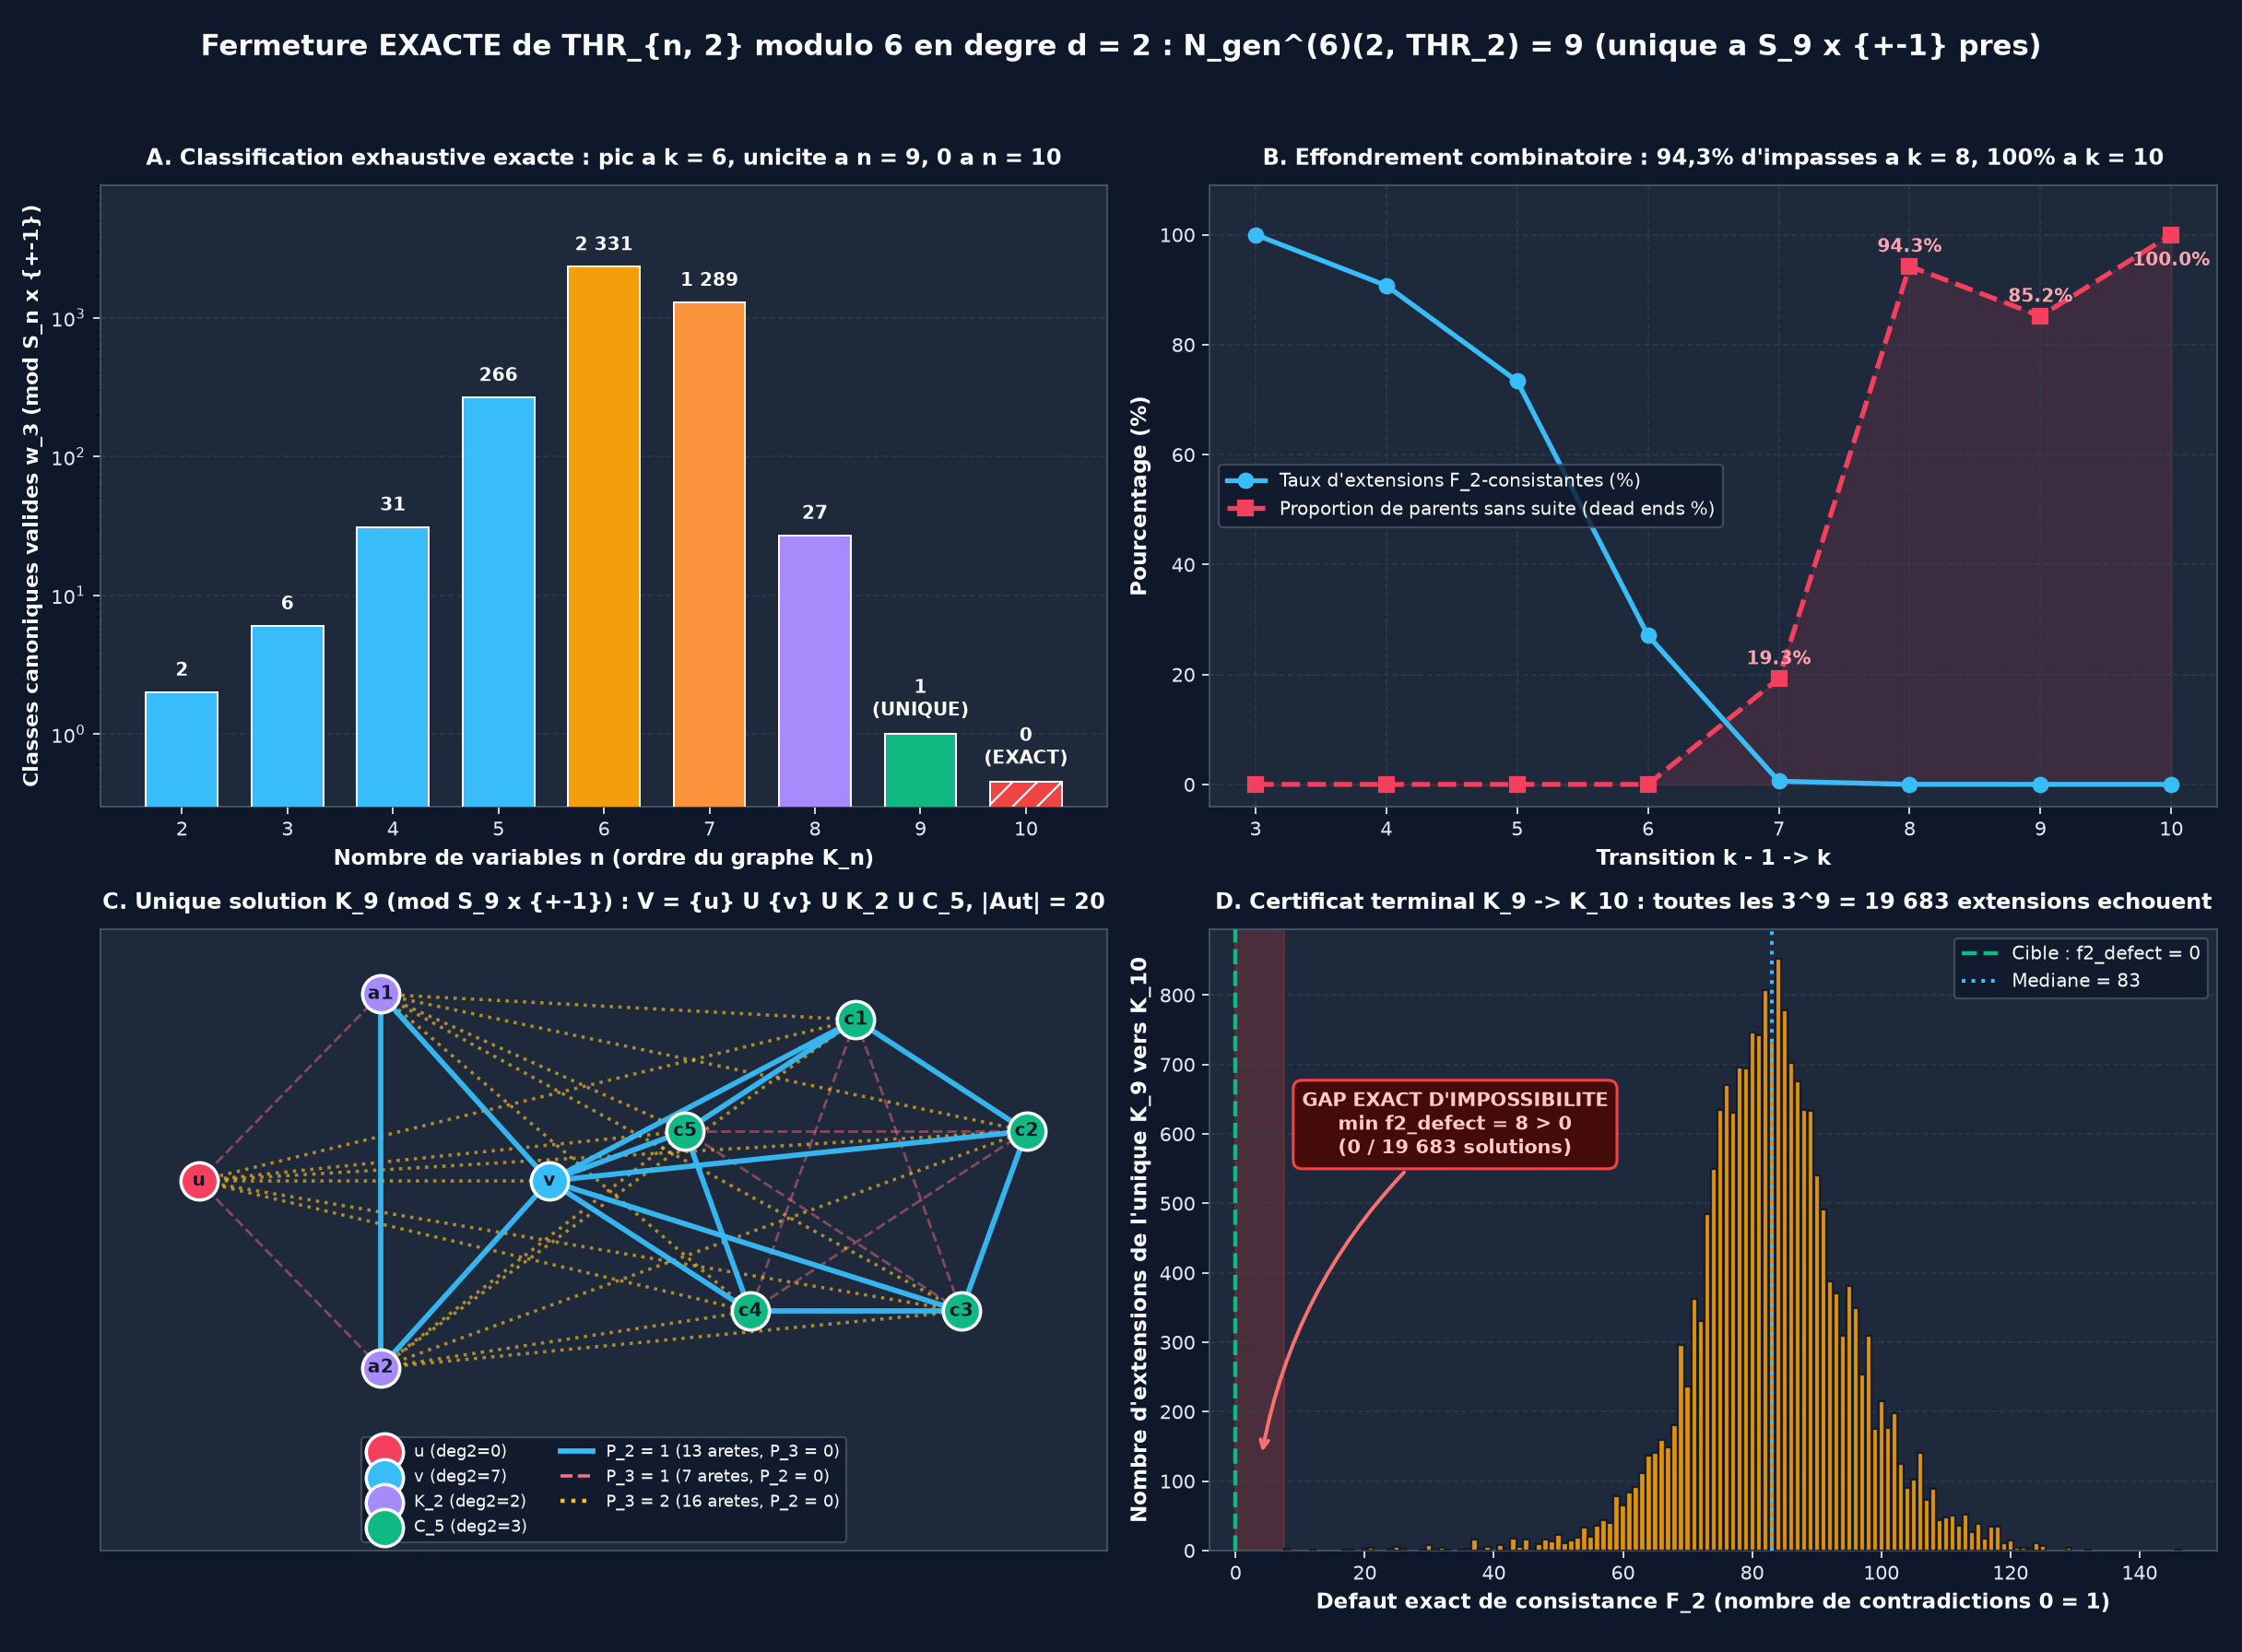
\includegraphics[width=0.92\textwidth]{../figures/thr2_mod6_exact_closure.png}
\caption{Exact hereditary closure of $\THR_{n,2}$ modulo $6$ at $n = 9$ (Theorem~\ref{thm:u1}), with unique canonical structure $V = \{u\} \sqcup \{v\} \sqcup K_2 \sqcup C_5$.}
\label{fig:u1}
\end{figure}

Using the same hereditary canonical engine accelerated by true-twin quotienting, we also obtain:
\begin{theorem}[Canonical Classification of Homogeneous Families of $\OR_n$ mod $6$ --- Theorem U2]
\label{thm:u2}
Among the three canonical homogeneous families of quadratic weak representations of $\OR_n$ modulo $6$:
\begin{itemize}[leftmargin=*,nosep]
  \item Family $V_0$ ($P_2$ homogeneous, $P_3$ homogeneous on weight-$1$ zeros): exact extinction at $n = 9$ ($4$ canonical classes, $0$ at $n = 10$).
  \item Family $W_{0,1}$ ($P_2$ homogeneous, $P_3$ with linear terms): exact extinction at $n = 10$ ($5$ canonical classes, $0$ at $n = 11$).
  \item Family $W_{1,1}$ ($P_2$ and $P_3$ with linear terms): exact extinction at $n = 10$ ($866$ canonical classes; $0 / 51.4 \times 10^6$ extensions at $n = 11$).
\end{itemize}
Additionally, canonical hereditary enumeration of quadratic $P_3$ without nonzero even-weight zeros ($6 \to 28 \to 119 \to 272 \to 109 \to 13 \to 0$, $0 / 4\,992$ extensions at $k = 8$) closes the mixed degree exactly:
\[
  \Ngen^{(6)}\bigl((1, 2), \OR\bigr) \;=\; 7 \;=\; 3p - 2 \qquad \bigl(\text{vs.\ } \Nsym^{(6)}((1, 2), \OR) = 5\bigr).
\]
\end{theorem}

%======================================================================
\section{Open Problems and Reproducibility}
\label{sec:open}
%======================================================================

Three main open problems emerge directly from this work:
\begin{enumerate}[leftmargin=*]
  \item \textbf{Tightening $8p - 7 \to 4p - 2$ on $m = 2p$:} Eliminating the factor-$2$ pairing loss on $U_1$ in Theorem~\ref{thm:d4} would close the gap between $4p - 2$ and $8p - 7$ (e.g., $18 \le \Ngen^{(10)}(2, \OR) \le 33$).
  \item \textbf{From $O(m^{3/2})$ to $O(m)$ on all semiprimes $m = pq$:} Resolving Conjecture~\ref{conj:lee} in full generality for odd semiprimes $m = pq$ requires overcoming the simultaneous high-rank regime $\min(r_p, r_q) = \Omega(p)$ isolated in Theorem~\ref{thm:d5}(4), likely by combining algebraic contraction with a non-Fourier bias argument over $\F_p \times \F_q$.
  \item \textbf{Mechanical verification in Lean~4:} A structured Lean~4 formalization of the core analytical proofs (Theorems~\ref{thm:g3pp}, \ref{thm:g5}, \ref{thm:d4}, and~\ref{thm:d5}) is included in the repository directory \texttt{lean/}, ready for compilation with Mathlib~4 via \texttt{lake build}, accompanied by an executable exact-arithmetic Python verifier (\texttt{lean/verify\_proof\_steps\_exact.py}) checking all finite lemmas and identities.
\end{enumerate}

All scripts, JSON logs, and figures are archived in the public repository.

\bibliographystyle{plain}
\bibliography{references}

\end{document}
